\documentclass[11pt]{amsart}
\usepackage[T1]{fontenc}\usepackage[utf8]{inputenc}\usepackage{lmodern}
\usepackage{amsmath,amssymb,amsfonts,amsthm,mathtools,graphicx,booktabs}
\usepackage{geometry}\usepackage{enumitem}\geometry{margin=1in}
\numberwithin{equation}{section}\setcounter{tocdepth}{3}\setcounter{secnumdepth}{3}
\newtheorem{theorem}{Theorem}[section]\newtheorem{proposition}[theorem]{Proposition}
\newtheorem{lemma}[theorem]{Lemma}\newtheorem{corollary}[theorem]{Corollary}
\usepackage[hidelinks]{hyperref}
\title[Three-State Gated Two-Harmonic Distributions]{Three-State Gated Two-Harmonic Distributions: Critical-Point Classification, Statistical Inference, Photonic Bands, and an Arithmetic Example}
\author{}\date{}
\begin{document}
\begin{abstract}
We study a gated family obtained by pushing uniform circle measure through two-frequency
trigonometric polynomials.  We prove an inverse-branch density formula, an absolutely
convergent resonant Bessel expansion, exact moment selection rules, a symmetry
classification, and a complete classification of multiple critical points for distinct
frequencies.  In particular, critical orders are at most four.  For i.i.d. observations
in a compact separated parameter chamber, we construct moment and empirical-
characteristic-function estimators, prove consistency and asymptotic normality, derive
the ECF sandwich covariance, establish parametric-bootstrap validity, and give exact or
conservative finite-sample confidence sets by distribution-function inversion.  Unknown
frequencies are treated separately as finite discrete model selection under an explicit
cross-model gap.  We derive a photonic tight-binding realization and identify a tunable
cubic transition in a published synthetic-frequency platform.  As a separate arithmetic
example, Möbius sampling with phase $\omega k\log k$ satisfies unconditional
quantitative Kolmogorov bounds, including an effective rate of order
$(\log\log N)(\log N)^{-1/4}$; random-index inference for a fixed finite prefix is
handled by hypergeometric inversion and Serfling bounds, without interpreting those
design intervals as rates for the infinite arithmetic limit.
\end{abstract}
\maketitle
\tableofcontents
\section{Introduction}\label{sec:introduction}
The experimental work of Dutt et al.\ \cite{DuttEtAl2019} provides the physical
motivation for the present study.  That work introduced direct band-structure
spectroscopy in a synthetic frequency dimension and demonstrated reconfigurable
long-range hopping, a photonic gauge phase, asymmetric bands, and direct access to the
density of states and its Van Hove singularities.  In particular, its two-drive
dispersion contains a first cosine harmonic and a phase-shifted higher harmonic.  At
gauge phase $\pi/2$, this is, up to an energy scale and reflection of quasimomentum,
precisely a function of the form
\begin{equation}
 \lambda\sin(r\theta)+\eta\cos(s\theta).
\label{eq:intro_two_harmonic}
\end{equation}
The relevance and experimental flexibility of this platform motivated us to ask for a
systematic probabilistic generalization of such dispersions: their complete value laws
under uniform quasimomentum, the singularities of those laws, the exact information
contained in their moments and characteristic functions, and the effect of mixing
distinct homogeneous gauge domains.

The present paper studies the first nontrivial gated version of this program.  Let
$\Theta$ be uniform on $[0,2\pi)$ and independent of $M$, where
\begin{equation}P(M=0)=1-q,\qquad P(M=1)=P(M=-1)=q/2.\label{eq:gate}\end{equation}
For positive $\lambda,\eta$ and coprime $r,s\in\mathbb N$, define
\begin{equation}X=\lambda M\sin(r\Theta)+\eta\cos(s\Theta).\label{eq:X}\end{equation}
Thus the model already has three gate states: two time-reversed active domains and one
inactive higher-harmonic domain.  The two-state model is the restriction
$M\in\{-1,1\}$, equivalently $q=1$.  A later extension may replace $M$ by an arbitrary
finite categorical gate, or allow several independently gated harmonics.  We do not
develop that larger model here, because its identifiability and degeneracy geometry
require a separate analysis.

As one example, the Möbius function supplies a deterministic sampling mechanism for this
probability law, but it does not define or restrict the probabilistic family.  It is a
particularly natural three-state gate because
\begin{equation}
 \mu(k)\in\{-1,0,1\},\qquad
 \operatorname{dens}\{\mu=0\}=1-\frac{6}{\pi^2},\qquad
 \operatorname{dens}\{\mu=\pm1\}=\frac{3}{\pi^2}.
 \label{eq:mobius_three_state_densities}
\end{equation}
The zero state records nonsquarefree integers, while the two active states record the
parity of the number of prime factors on the squarefree integers.  Thus Möbius supplies
the same gate weights as \eqref{eq:gate} with $q=6/\pi^2$, together with substantial
known multiplicative and equidistribution structure.  The gate and phase are not assumed
independent at finite sample size; the arithmetic theorem proves that the corresponding
mixture nevertheless emerges asymptotically.

The circle-pushforward theory and its physical DOS interpretation remain meaningful
for laboratory quasimomentum samples, random categorical gates, other arithmetic weights,
and deterministic sequences satisfying appropriate joint equidistribution conditions.
The four layers of the paper are logically separate.  Sections~\ref{sec:probability}--
\ref{sec:limits} concern the exact circle pushforward; Section~\ref{sec:inference}
assumes an explicitly i.i.d. sample; Sections~\ref{sec:arithmetic} and
\ref{sec:numerics} concern a deterministic arithmetic sequence and use no i.i.d.
calibration; Sections~\ref{sec:dutt}--\ref{sec:physics} concern homogeneous Bloch bands
and their uniform-quasimomentum DOS.  No conclusion is transferred between these four
settings without a separately stated theorem.
Circle pushforwards and density-of-states singularities are standard; see
\cite{VanHove1953,ClassenBetouras2025}.  Our contribution is the integrated analysis of
\eqref{eq:X}, including an explicit finite degeneracy set for every coprime frequency
pair and a proof that no critical order above four can occur.  Möbius sampling is treated
only as a subsequent arithmetic example.  The literature audit accompanying this paper does not justify claiming that trigonometric
pushforwards or higher-order Van Hove singularities themselves are new.  A subscriber
MathSciNet audit and a complete Google Scholar exact-formula search remain pending.
\section{Probability law}\label{sec:probability}
Put $h(\theta)=\lambda\sin(r\theta)+\eta\cos(s\theta)$.
\begin{lemma}\label{lem:mixture}
The conditional laws for $M=1$ and $M=-1$ coincide.  Hence
\begin{equation}\mathcal L(X)=(1-q)(\eta\cos(s\Theta))_\#m+q(h(\Theta))_\#m,\label{eq:two_mixture}\end{equation}
where $m$ is normalized circle measure.
\end{lemma}
\begin{proof}Use $\theta\mapsto-\theta$.\end{proof}
\begin{theorem}\label{thm:density}
For every
\begin{equation}
 x\notin \operatorname{CritVal}(h)\cup\{-\eta,\eta\},
 \label{eq:density_regular_set}
\end{equation}
the density is given pointwise by
\begin{equation}f_X(x)=\frac{(1-q){\bf1}_{|x|<\eta}}{\pi\sqrt{\eta^2-x^2}}
+\frac q{2\pi}\sum_{h(\theta)=x}\frac1{|h'(\theta)|}.\label{eq:density}\end{equation}
If $q>0$, then
\begin{equation}
 \operatorname{supp}(X)=[\min h,\max h].
 \label{eq:density_support_active}
\end{equation}
If $q=0$, then
\begin{equation}
 \operatorname{supp}(X)=[-\eta,\eta].
 \label{eq:density_support_inactive}
\end{equation}
\end{theorem}
\begin{proof}
Partition the circle at the finitely many critical phases of $h$.  On each resulting
monotonicity interval, the change-of-variables formula gives the active term in
\eqref{eq:density}; the arcsine change of variables gives the first term.  These formulas
are pointwise valid away from the active critical values and the arcsine edges.

The image of the circle under $h$ is the interval $[\min h,\max h]$.  If
$\cos(s\theta)=\pm1$, then
\begin{equation}
 \frac{h(\theta)+h(-\theta)}2=\eta\cos(s\theta)=\pm\eta.
 \label{eq:active_support_contains_arcsine_edges}
\end{equation}
Because the image is an interval, it contains both $-\eta$ and $\eta$, and hence it
contains $[-\eta,\eta]$.  Therefore, when $q>0$, the support of the mixture is the active
support $[\min h,\max h]$.  When $q=0$, only the arcsine component remains, whose support
is $[-\eta,\eta]$.
\end{proof}
\section{Characteristic function and moments}\label{sec:characteristic}
\begin{theorem}\label{thm:cf}
For every real $t$,
\begin{equation}\phi_X(t)=(1-q)J_0(\eta t)+q\sum_{\ell\in\mathbb Z}
i^{r\ell}J_{s\ell}(\lambda t)J_{r\ell}(\eta t),\label{eq:cf}\end{equation}
and the series converges absolutely and locally uniformly.
\end{theorem}
\begin{proof}Apply the Jacobi--Anger expansions \cite{DLMF2026}; circle integration
retains precisely $mr+ns=0$, hence $(m,n)=(s\ell,-r\ell)$.  The standard factorial
bounds for integer-order Bessel functions make both Jacobi--Anger series absolutely and
uniformly convergent when $t$ ranges over a compact set.  Explicitly, for $n\ge0$ and
$|x|\le T$, the defining series and $(n+j)!\ge n!j!$ give
\begin{equation}
 |J_n(x)|\le \frac{(T/2)^n}{n!}
 \sum_{j\ge0}\frac{(T^2/4)^j}{(j!)^2}
 \le \frac{(T/2)^n}{n!}e^{T^2/4},
 \qquad |J_{-n}(x)|=|J_n(x)|.
 \label{eq:bessel_uniform_factorial_bound}
\end{equation}
The Weierstrass test therefore applies to both Jacobi--Anger series and their product.
Fubini's theorem permits termwise circle integration, and the retained one-dimensional
subseries is absolutely and locally uniformly convergent.
\end{proof}
For $a,b\ge0$, set $I_{a,b}=\int\sin^a(r\theta)\cos^b(s\theta)\,dm$.
\begin{proposition}\label{prop:resonance}
\begin{equation}I_{a,b}=\frac1{(2i)^a2^b}\sum_{j=0}^a\sum_{k=0}^b
(-1)^j\binom aj\binom bk{\bf1}_{r(a-2j)+s(b-2k)=0}.\label{eq:resonance}\end{equation}
Thus all moments and cumulants are finite explicit sums.  If $r\ne s$,
\begin{align}E[X^2]&=(\eta^2+q\lambda^2)/2,\label{eq:m2}\\
E[X^4]&=3\eta^4/8+q(3\lambda^4/8+3\lambda^2\eta^2/2).\label{eq:m4}
\end{align}
\end{proposition}
\begin{proof}
The exponential identities
\begin{equation}
 \sin^a(r\theta)=\frac{1}{(2i)^a}
 \sum_{j=0}^a(-1)^j\binom aj e^{ir(a-2j)\theta},
 \qquad
 \cos^b(s\theta)=\frac{1}{2^b}
 \sum_{k=0}^b\binom bk e^{is(b-2k)\theta}
 \label{eq:moment_exponential_expansions}
\end{equation}
give \eqref{eq:resonance} after integration, because only the zero Fourier frequency
survives.  Expanding powers of \eqref{eq:X} and using
$E[M^j]=0$ for odd $j$ and $E[M^j]=q$ for positive even $j$ reduces every moment to
these finite sums.  Finally,
\begin{equation}
 I_{2,0}=I_{0,2}=\frac12,
 \qquad I_{4,0}=I_{0,4}=\frac38,
 \qquad I_{2,2}=\frac14\quad(r\ne s),
 \label{eq:low_order_harmonic_integrals}
\end{equation}
which gives \eqref{eq:m2} and \eqref{eq:m4}.
\end{proof}
\section{Symmetry and identifiability}\label{sec:symmetry}
\begin{theorem}\label{thm:symmetry}
For $q\lambda\eta>0$ and reduced frequencies, $X$ is symmetric if and only if $s$ is odd.
If $s$ is even, then $r$ is odd and
\begin{equation}E[X^{r+s}]=q\binom{r+s}{s}2^{1-r-s}(-1)^{s/2}\lambda^s\eta^r\ne0.\label{eq:oddmoment}\end{equation}
\end{theorem}
\begin{proof}
Suppose first that $s$ is odd.  If $r$ is odd, the measure-preserving map
$\theta\mapsto\theta+\pi$ changes the signs of both harmonics.  If $r$ is even, the
map $\theta\mapsto\pi-\theta$ does so.  Hence the law is symmetric.

Now let $s$ be even.  Coprimality forces $r$ to be odd, so $n=r+s$ is odd.  In the
binomial expansion of $E[X^n]$, terms with an odd power $a$ of the sine harmonic vanish
because $E[M^a]=0$, and the term $a=0$ is the mean of an odd power of a cosine.  For
positive even $a$ put $b=n-a$.  A nonzero Fourier contribution to $I_{a,b}$ requires
integers $j,k$ such that
\begin{equation}
 r(a-2j)+s(b-2k)=0.
 \label{eq:symmetry_resonance_equation}
\end{equation}
Coprimality gives $a-2j=sL$ and $b-2k=-rL$.  Here $L$ is odd, while
$s|L|\le a$, $r|L|\le b$, and $a+b=r+s$; consequently $L=\pm1$ and necessarily
$(a,b)=(s,r)$.  The two retained Fourier terms in \eqref{eq:resonance} give
\begin{equation}
 I_{s,r}=2^{1-r-s}(-1)^{s/2}.
 \label{eq:unique_odd_resonance}
\end{equation}
Multiplication by the binomial coefficient, amplitudes, and $E[M^s]=q$ proves
\eqref{eq:oddmoment}.  This nonzero odd moment excludes symmetry.
\end{proof}
\begin{proposition}\label{prop:identifiability}
Fix distinct positive integers $r$ and $s$, and let
\begin{equation}
 \mathcal P=(0,\infty)^2\times(0,1)
 \label{eq:identifiability_parameter_space}
\end{equation}
be the parameter space for $p=(\lambda,\eta,q)$.  For
$h_p(\theta)=\lambda\sin(r\theta)+\eta\cos(s\theta)$, fix
$p_0=(\lambda_0,\eta_0,q_0)\in\mathcal P$.  Suppose that there exist an open
neighborhood $U\subset\mathcal P$ of $p_0$ and a number $\delta>0$ such that
\begin{equation}
 \operatorname{dist}\bigl(\{-\eta,\eta\},\operatorname{CritVal}(h_p)\bigr)>\delta
 \qquad\text{for every }p=(\lambda,\eta,q)\in U.
 \label{eq:identifiability_edge_separation}
\end{equation}
Then $p\mapsto\mathcal L(X_p)$ is injective on a possibly smaller neighborhood of
$p_0$.  In particular, $(\lambda,\eta,q)$ is locally identifiable.  Once $\eta$ has
been recovered from the law, put
\begin{equation}
 A=2E[X^2]-\eta^2,
 \qquad
 B=\frac83\left(E[X^4]-\frac{3\eta^4}{8}\right).
 \label{eq:identifiability_observables}
\end{equation}
Then
\begin{equation}\lambda^2=B/A-4\eta^2,\qquad q=A/\lambda^2.\label{eq:moment_identification}\end{equation}
\end{proposition}
\begin{proof}
Because $0<q<1$, the arcsine component has positive mass.  By
\eqref{eq:identifiability_edge_separation}, the active density has no critical-value
singularity in the $\delta$-neighborhood of either arcsine edge.  Hence the law has two
isolated square-root singularities at the symmetric locations $-\eta$ and $\eta$ that
persist throughout $U$.  Their locations determine the positive parameter $\eta$.

The second and fourth moments are observables of the law.  Equations \eqref{eq:m2} and
\eqref{eq:m4} give
\begin{equation}
 A=q\lambda^2,
 \qquad
 B=q\lambda^4+4q\lambda^2\eta^2
   =A(\lambda^2+4\eta^2).
 \label{eq:identifiability_AB}
\end{equation}
Since $q>0$ and $\lambda>0$, one has $A>0$.  Therefore the law determines
$\lambda^2=B/A-4\eta^2$, and positivity selects the unique value $\lambda>0$.
It then determines $q=A/\lambda^2$.  Thus any two parameters in a sufficiently small
neighborhood of $p_0$ with the same law have identical $\eta$, $\lambda$, and $q$.
\end{proof}
Degeneracies include $q=0$, $\lambda=0$, and $r=s$, the latter reducing to an arcsine
component of radius $\sqrt{\lambda^2+\eta^2}$.
\section{Critical values}\label{sec:critical}
\subsection{The one-dimensional Van Hove mechanism}\label{subsec:van_hove_summary}
For a one-dimensional band $\varepsilon(k)$ sampled with uniform quasimomentum, the
density of states is the pushforward density
\begin{equation}
 g(E)=\frac{1}{2\pi}\sum_{\varepsilon(k)=E}\frac{1}{|\varepsilon'(k)|}.
 \label{eq:van_hove_dos}
\end{equation}
It is smooth at regular energies but becomes singular at a critical energy
$E_c=\varepsilon(k_c)$ where $\varepsilon'(k_c)=0$.  At an ordinary quadratic band
edge, $\varepsilon(k)-E_c$ is proportional to $(k-k_c)^2$, and hence
$g(E)$ diverges on one side as $|E-E_c|^{-1/2}$.  If the first nonzero derivative has
order $m>2$, the band is locally flatter and the divergence strengthens to
$|E-E_c|^{1/m-1}$.  This critical-point mechanism goes back to Van Hove
\cite{VanHove1953}; higher-order versions are now standard objects of band theory
\cite{ClassenBetouras2025}.  Our new question is not whether such singularities exist,
but exactly which orders and tuning ratios are possible in the constrained
two-frequency family \eqref{eq:degeneracy_h}.

\begin{theorem}\label{thm:singularity}
Assume $q>0$.  If $h^{(1)}(\theta_0)=\cdots=h^{(m-1)}(\theta_0)=0$ and
$h^{(m)}(\theta_0)\ne0$, put $x_0=h(\theta_0)$ and
$a_m=h^{(m)}(\theta_0)/m!$.  On every locally accessible side of $x_0$, the
contribution of this phase to the active-branch density satisfies
\begin{equation}
 f_{\theta_0}(x)\sim
 \frac{qN_m}{2\pi m|a_m|^{1/m}}|x-x_0|^{1/m-1},
 \label{eq:singularity_prefactor}
\end{equation}
where $N_m=1$ for odd $m$ and $N_m=2$ for even $m$.  In the even case the
accessible side is $a_m(x-x_0)>0$, and the phase contributes nothing on the other
side sufficiently close to $x_0$.  In particular, the exponent is
\begin{equation}|x-h(\theta_0)|^{1/m-1}.\label{eq:singularity_exponent}\end{equation}
For even $m$ it is one-sided; for odd $m$ it occurs on both sides.
\end{theorem}
\begin{proof}
Write $u=\theta-\theta_0$.  Taylor's theorem gives
\begin{equation}
 h(\theta_0+u)-x_0=a_mu^m\{1+o(1)\},\qquad
 h'(\theta_0+u)=ma_mu^{m-1}\{1+o(1)\}.
 \label{eq:singularity_taylor_pair}
\end{equation}
Along each accessible inverse branch,
\begin{equation}
 |u|=|a_m|^{-1/m}|x-x_0|^{1/m}\{1+o(1)\},
 \quad
 \frac1{|h'(\theta_0+u)|}
 =\frac{|x-x_0|^{1/m-1}}{m|a_m|^{1/m}}\{1+o(1)\}.
 \label{eq:singularity_inverse_derivative}
\end{equation}
An odd power has one local real inverse branch on each side; an even power has two on
the side $a_m(x-x_0)>0$ and none on the other side.  Multiplication by the active mass
$q/(2\pi)$ and the corresponding branch count $N_m$ proves
\eqref{eq:singularity_prefactor}.
\end{proof}
If $q=0$, the active component in \eqref{eq:two_mixture} has mass zero and contributes no
density.

\begin{theorem}[Complete multiple-critical-point classification]
\label{thm:complete_degeneracy}
Let $r$ and $s$ be distinct coprime positive integers and let $\lambda,\eta>0$.
Every critical point of
\begin{equation}
 h(\theta)=\lambda\sin(r\theta)+\eta\cos(s\theta)
 \label{eq:degeneracy_h}
\end{equation}
has order $2$, $3$, or $4$.  All points of order at least $3$ are obtained as follows.

Away from the quartic case below, their phases are precisely the solutions of
\begin{equation}
 (r+s)\cos((r-s)\theta)
 =
 (r-s)\cos((r+s)\theta)
 \label{eq:degeneracy_phase_equation}
\end{equation}
for which
\begin{equation}
 \frac{\lambda}{\eta}
 =
 \frac{s\sin(s\theta)}{r\cos(r\theta)}>0.
 \label{eq:cubic_ratio}
\end{equation}
Every such point has order $3$ and density exponent $-2/3$.

An order-$4$ point exists if and only if
\begin{equation}
 r\ \text{is odd},\qquad s\ \text{is even},\qquad
 \frac{\lambda}{\eta}=\frac{s^2}{r^2}.
 \label{eq:quartic_condition}
\end{equation}
For positive amplitudes exactly one of $\theta=\pi/2$ and $\theta=3\pi/2$ is the
quartic phase.  Its density exponent is $-3/4$.  Consequently, for each fixed
$(r,s)$ the set of amplitude ratios at which the number of critical points can change is
finite and explicitly computable from \eqref{eq:degeneracy_phase_equation} and
\eqref{eq:quartic_condition}.
\end{theorem}
\begin{proof}
The first four derivatives are
\begin{align}
 h'&=\lambda r\cos(r\theta)-\eta s\sin(s\theta),
 \label{eq:degeneracy_d1}\\
 h''&=-\lambda r^2\sin(r\theta)-\eta s^2\cos(s\theta),
 \label{eq:degeneracy_d2}\\
 h'''&=-\lambda r^3\cos(r\theta)+\eta s^3\sin(s\theta),
 \label{eq:degeneracy_d3}\\
 h^{(4)}&=\lambda r^4\sin(r\theta)+\eta s^4\cos(s\theta).
 \label{eq:degeneracy_d4}
\end{align}
The determinant of the homogeneous linear system in $(\lambda,\eta)$ given by
$h'=h''=0$ vanishes precisely when
\begin{equation}
 s\cos(r\theta)\cos(s\theta)
 +r\sin(r\theta)\sin(s\theta)=0.
 \label{eq:degeneracy_determinant}
\end{equation}
The product-to-sum identities turn \eqref{eq:degeneracy_determinant} into
\eqref{eq:degeneracy_phase_equation}.  If $\cos(r\theta)\ne0$, the first derivative
then gives \eqref{eq:cubic_ratio}.  Conversely, a phase satisfying these two equations
makes both \eqref{eq:degeneracy_d1} and \eqref{eq:degeneracy_d2} vanish.

At any critical point, set
$C=\lambda r\cos(r\theta)=\eta s\sin(s\theta)$.  Equation
\eqref{eq:degeneracy_d3} gives
\begin{equation}
 h'''(\theta)=(s^2-r^2)C.
 \label{eq:third_derivative_reduction}
\end{equation}
Because $r\ne s$, a multiple critical point is cubic unless $C=0$.  In the latter
case, positivity of the amplitudes implies
\begin{equation}
 \cos(r\theta)=0,\qquad \sin(s\theta)=0.
 \label{eq:quartic_phase_conditions}
\end{equation}
For coprime frequencies, \eqref{eq:quartic_phase_conditions} is solvable precisely when
$s$ is even; then $r$ is odd and the only phases modulo $2\pi$ are $\pi/2$ and
$3\pi/2$.  At these phases, $h''=0$ has a positive-amplitude solution at exactly one
of the two phases.  Indeed,
\begin{equation}
 \frac{\lambda}{\eta}
 =-\frac{s^2\cos(s\theta)}{r^2\sin(r\theta)}.
 \label{eq:quartic_ratio_with_sign}
\end{equation}
The cosine has the same sign at the two candidate phases, whereas the sine has opposite
signs.  Exactly one ratio is therefore positive, and its modulus is $s^2/r^2$.

Finally, using $h''=0$ in \eqref{eq:degeneracy_d4} gives
\begin{equation}
 h^{(4)}(\theta)
 =\lambda r^2(r^2-s^2)\sin(r\theta)\ne0.
 \label{eq:fourth_derivative_nonzero}
\end{equation}
Thus the remaining point is quartic and no order above four is possible.  The left-hand
side of \eqref{eq:degeneracy_phase_equation} is a nonzero trigonometric polynomial of
degree $r+s$, so it has only finitely many phases.  Away from their associated ratios,
the implicit-function theorem preserves the number of critical points.
\end{proof}

General higher-order Van Hove classification and catastrophe-theory normal forms are
established topics \cite{ClassenBetouras2025}.  Theorem~\ref{thm:complete_degeneracy}
is instead an exact global classification within the constrained two-frequency family.
Its novelty status remains subject to the source-by-source audit accompanying this paper.

For $(r,s)=(2,1)$ and $\rho=\eta/\lambda$, stationary points satisfy
\begin{equation}u_\pm=\frac{-\rho\pm\sqrt{\rho^2+32}}8,\qquad
c_\pm=\lambda\sqrt{1-u_\pm^2}(2u_\pm+\rho).\label{eq:initial_critical}\end{equation}
The $u_-$ branch exists for $\rho\le2$; at $\rho=2$ it is cubic and gives exponent
$-2/3$.  For $\rho=1/4$ the six singular values are
$\pm1.1805175473$, $\pm0.8273102715$, and $\pm0.25$.
\section{Limits}\label{sec:limits}
Scaling $(\lambda,\eta)$ scales $X$.  As $q\to0$ or $\lambda\to0$ one obtains the
arcsine law of radius $\eta$.  As $\eta\to0$, an atom of mass $1-q$ at zero remains.
\begin{proposition}\label{prop:frequency_limit}
If reduced pairs $(r_n,s_n)$ escape every finite set, the circle measures
$\theta\mapsto(r_n\theta,s_n\theta)$ converge weakly to Haar measure on the two-torus;
the branch limit is therefore the convolution of independent arcsine laws.
\end{proposition}
\begin{proof}
For $(u,v)\in\mathbb Z^2$, the $(u,v)$ Fourier coefficient of the image measure is
\begin{equation}
 \frac{1}{2\pi}\int_0^{2\pi}
 e^{i(ur_n+vs_n)\theta}\,d\theta
 =\mathbf 1_{\{ur_n+vs_n=0\}}.
 \label{eq:subtorus_fourier_coefficient}
\end{equation}
For fixed $(u,v)\ne(0,0)$, the last equality can hold for at most one coprime positive
pair $(r_n,s_n)$.  Hence every nonconstant Fourier coefficient tends to zero, which is
the Fourier characterization of Haar convergence on the two-torus.  Applying the
continuous map $(x,y)\mapsto\lambda\sin x+\eta\cos y$ gives the stated convolution.
\end{proof}
\section{An arithmetic example: Möbius sampling}\label{sec:arithmetic}
The role of Möbius in this section is illustrative but nontrivial.  Unlike an artificial
i.i.d. categorical draw, it is a deterministic three-state sequence whose state
frequencies are known and whose signed squarefree structure is arithmetic.  It therefore
tests whether the same gated law can arise from structured deterministic sampling rather
than from the independence assumption used in \eqref{eq:gate}.
Define
\begin{equation}F(k)=\lambda\mu(k)\sin(r\omega k\log k)+\eta\cos(s\omega k\log k).\label{eq:F}\end{equation}
\begin{theorem}\label{thm:arithmetic}
For every fixed $\omega\ne0$, the empirical measures $N^{-1}\sum_{k\le N}\delta_{F(k)}$
converge weakly to \eqref{eq:two_mixture} with $q=6/\pi^2$.
\end{theorem}
\begin{proof}
For $z\in\{-1,0,1\}$, let
\begin{equation}
 E_z=\{n\in\mathbb N:\mu(n)=z\}.
 \label{eq:mobius_level_sets}
\end{equation}
Since the Möbius function is multiplicative, each $E_z$ is a one-function level set and
therefore belongs to the class $\mathcal D^{(1)}$ in Definition~1.3 of
\cite{BergelsonKulagaPrzymusLemanczykRichter2019}.  The squarefree-density theorem gives
\begin{equation}
 d(E_{-1})+d(E_1)=\frac6{\pi^2},
 \qquad
 d(E_0)=1-\frac6{\pi^2}.
 \label{eq:mobius_level_density_sum}
\end{equation}
The prime number theorem is equivalent to
$N^{-1}\sum_{n\le N}\mu(n)\to0$, and hence
\begin{equation}
 d(E_{-1})=d(E_1)=\frac3{\pi^2}.
 \label{eq:mobius_signed_level_densities}
\end{equation}
Thus every $E_z$ has an existing positive density.  Proposition~3.2 on p.~2591 of the
cited paper then places each $E_z$ in $\mathcal E_{\mathrm{c.pt.}}^{(1)}$, exactly one
of the two set classes admitted by its Theorem~4.1 on pp.~2607--2608.

Set
\begin{equation}
 h_\omega(t)=\frac{\omega}{2\pi}t\log t.
 \label{eq:hardy_phase}
\end{equation}
For $\omega\ne0$, this function belongs to the logarithmico-exponential Hardy field.  It
has polynomial growth because $|h_\omega(t)|/t^2\to0$.  Let
$P\in\mathbb Q[t]$.  If $\deg P\ge2$, then
$|h_\omega(t)-P(t)|$ is asymptotic to the modulus of the leading term of $P$.  If
$\deg P\le1$, then
\begin{equation}
 |h_\omega(t)-P(t)|\sim\frac{|\omega|}{2\pi}t\log t.
 \label{eq:hardy_phase_linear_separation}
\end{equation}
In both cases,
\begin{equation}
 \frac{|h_\omega(t)-P(t)|}{\log^2t}\longrightarrow\infty.
 \label{eq:hardy_phase_boshernitzan_condition}
\end{equation}
All hypotheses of Theorem~4.1 of
\cite{BergelsonKulagaPrzymusLemanczykRichter2019} therefore hold for each of the three
sets $E_z$.  If $E_z=\{n_{z,1}<n_{z,2}<\cdots\}$, the sequence
$h_\omega(n_{z,j})$ is uniformly distributed modulo one.  Equivalently,
$\omega n_{z,j}\log n_{z,j}$ is uniformly distributed modulo $2\pi$.

Let $\psi$ be bounded and continuous, and put
\begin{equation}
 H_z(\theta)=\psi\bigl(\lambda z\sin(r\theta)+\eta\cos(s\theta)\bigr).
 \label{eq:arithmetic_test_functions}
\end{equation}
Uniform distribution on $E_z$ and the density of $E_z$ give
\begin{equation}
 \frac1N\sum_{\substack{k\le N\\k\in E_z}}\psi(F(k))
 \longrightarrow
 d(E_z)\frac1{2\pi}\int_0^{2\pi}H_z(\theta)\,d\theta.
 \label{eq:conditional_level_pushforward}
\end{equation}
Summing \eqref{eq:conditional_level_pushforward} over $z=-1,0,1$, using
\eqref{eq:mobius_signed_level_densities}, and applying Lemma~\ref{lem:mixture} yields
\begin{equation}
 \frac1N\sum_{k\le N}\psi(F(k))
 \longrightarrow
 \left(1-\frac6{\pi^2}\right)\int\psi\,d(\eta\cos(s\Theta))_\#m
 +\frac6{\pi^2}\int\psi\,d(h(\Theta))_\#m.
 \label{eq:arithmetic_weak_limit_test_function}
\end{equation}
This is the asserted weak convergence.
\end{proof}

\subsection{Quantitative Kolmogorov discrepancy}
\label{subsec:quantitative_arithmetic_discrepancy}
The qualitative theorem admits an unconditional quantitative strengthening.  Define
\begin{equation}
 \mathcal F_\infty(x)
 =\left(1-\frac6{\pi^2}\right)
   \frac1{2\pi}\operatorname{meas}\{\theta:\eta\cos(s\theta)\le x\}
 +\frac6{\pi^2}\frac1{2\pi}\operatorname{meas}\{\theta:h(\theta)\le x\}
 \label{eq:arithmetic_limiting_cdf}
\end{equation}
and
\begin{equation}
 \mathfrak D_N
 =\sup_{x\in\mathbb R}
 \left|\frac1N\#\{k\le N:F(k)\le x\}-\mathcal F_\infty(x)\right|.
 \label{eq:arithmetic_kolmogorov_discrepancy}
\end{equation}

\begin{theorem}[Quantitative arithmetic discrepancy]
\label{thm:quantitative_arithmetic_discrepancy}
Fix $\lambda,\eta>0$, positive integers $r,s$, and $\omega\ne0$.  For every $A>0$,
\begin{equation}
 \mathfrak D_N\ll_{A,\lambda,\eta,r,s,\omega}(\log N)^{-A},
 \label{eq:arithmetic_arbitrary_log_rate}
\end{equation}
where the implied constant is ineffective.  One also has the effective estimate
\begin{equation}
 \mathfrak D_N\ll_{\lambda,\eta,r,s,\omega}
 \frac{\log\log N}{(\log N)^{1/4}}.
 \label{eq:arithmetic_effective_log_rate}
\end{equation}
Both estimates hold for all sufficiently large $N$ and use no unproved
number-theoretic hypothesis.  Effectivity in \eqref{eq:arithmetic_effective_log_rate}
means that the implied constant and threshold are computable in principle; no numerical
value for either is asserted here.
\end{theorem}

Write $e(t)=\exp(2\pi i t)$ and, for $a\in\mathbb R$, set
\begin{align}
 U_a(N)&=\sum_{n\le N}e(a n\log n),
 \label{eq:arithmetic_unweighted_sum}\\
 Q_a(N)&=\sum_{n\le N}\mu(n)^2e(a n\log n),
 \label{eq:arithmetic_squarefree_sum}\\
 M_a(N)&=\sum_{n\le N}\mu(n)e(a n\log n).
 \label{eq:arithmetic_mobius_sum}
\end{align}

\begin{lemma}
\label{lem:arithmetic_unweighted_bound}
For $a\ne0$,
\begin{equation}
 U_a(N)\ll\left(|a|^{1/2}+|a|^{-1/2}\right)N^{1/2}+1.
 \label{eq:arithmetic_unweighted_bound}
\end{equation}
\end{lemma}
\begin{proof}
On $X<n\le2X$, the second derivative of $a t\log t$ has modulus between
$|a|/(2X)$ and $|a|/X$.  The van der Corput second-derivative estimate
\cite[Chapter~2]{GrahamKolesnik1991} gives
\begin{equation}
 \sum_{X<n\le2X}e(a n\log n)
 \ll |a|^{1/2}X^{1/2}+|a|^{-1/2}X^{1/2}.
 \label{eq:arithmetic_dyadic_unweighted_bound}
\end{equation}
Summation over dyadic intervals proves \eqref{eq:arithmetic_unweighted_bound}.
\end{proof}

\begin{lemma}
\label{lem:arithmetic_squarefree_bound}
For $a\ne0$ and $N$ sufficiently large in terms of $a$,
\begin{equation}
 Q_a(N)\ll
 |a|^{1/4}N^{3/4}+|a|^{-1/2}N^{1/2}+N^{1/2}.
 \label{eq:arithmetic_squarefree_bound}
\end{equation}
For every fixed $c,C>0$, the estimate is uniform when
$c\le|a|\le(\log N)^C$.
\end{lemma}
\begin{proof}
Use
\begin{equation}
 \mu(n)^2=\sum_{d^2\mid n}\mu(d).
 \label{eq:arithmetic_squarefree_identity}
\end{equation}
Split the resulting $d$-sum at $1\le Y\le N^{1/2}$.  For $d\le Y$, apply the
second-derivative estimate to
\begin{equation}
 g_d(t)=a d^2t\log(d^2t),
 \qquad g_d''(t)=\frac{a d^2}{t}.
 \label{eq:arithmetic_squarefree_inner_phase}
\end{equation}
After dyadic subdivision,
\begin{equation}
 \sum_{m\le N/d^2}e(a d^2m\log(d^2m))
 \ll |a|^{1/2}N^{1/2}
 +\frac{N^{1/2}}{|a|^{1/2}d^2}+1.
 \label{eq:arithmetic_squarefree_inner_bound}
\end{equation}
The range $d>Y$ contributes at most $O(N/Y)$.  Consequently,
\begin{equation}
 Q_a(N)\ll
 Y|a|^{1/2}N^{1/2}+|a|^{-1/2}N^{1/2}+Y+\frac NY.
 \label{eq:arithmetic_squarefree_optimization}
\end{equation}
Taking $Y$ to be the nearest admissible integer to
$|a|^{-1/4}N^{1/4}$ proves the result.
\end{proof}

\begin{proposition}
\label{prop:arithmetic_mobius_nlogn}
Fix $B>0$.  Uniformly for $|a|\le(\log N)^B$,
\begin{equation}
 M_a(N)\ll_B N(\log N)^{-1/4}+(1+|a|)N^{2/3},
 \label{eq:arithmetic_effective_mobius_nlogn}
\end{equation}
with an effective implied constant.  For every $A>0$,
\begin{equation}
 M_a(N)\ll_{A,B} N(\log N)^{-A}+(1+|a|)N^{2/3},
 \label{eq:arithmetic_strong_mobius_nlogn}
\end{equation}
where the implied constant is ineffective.
\end{proposition}
\begin{proof}
We use Theorem~1.1(i) and (iv) of
Matom\"aki, Shao, Tao, and Ter\"av\"ainen
\cite{MatomakiShaoTaoTeravainen2023}.  Their theorem is uniform over polynomial
phases of fixed degree on intervals $(X,X+H]$ with
$H\ge X^{5/8+\varepsilon}$ for an arbitrary logarithmic saving and with
$H\ge X^{3/5+\varepsilon}$ for the effective saving $(\log X)^{-1/4}$.

Partition $(X,2X]$ into full intervals $I=(y,y+H]$ with
$H=\lfloor X^{2/3}\rfloor$.  Keep a possible final interval of length less than $H$
separate and bound it trivially.  On a full interval let $P_y$ be the cubic Taylor
polynomial of $a t\log t$ at $y$.  Since
\begin{equation}
 \frac{d^4}{dt^4}(a t\log t)=\frac{2a}{t^3},
 \label{eq:arithmetic_fourth_derivative_nlogn}
\end{equation}
Taylor's theorem gives
\begin{equation}
 \sup_{t\in I}|a t\log t-P_y(t)|
 \ll |a|\frac{H^4}{X^3}\ll |a|X^{-1/3}.
 \label{eq:arithmetic_taylor_remainder}
\end{equation}
Replacing the phase by $P_y$ therefore costs $O(|a|HX^{-1/3})$ on $I$.

Choose a fixed $0<\varepsilon<1/24$.  Uniformly for $X\le y\le2X$ and all
sufficiently large $X$,
\begin{equation}
 y^{5/8+\varepsilon}\le H\le y^{1-\varepsilon}.
 \label{eq:arithmetic_short_interval_range}
\end{equation}
This verifies the hypotheses of both cited parts.  Polynomial phases of degree at most
three arise from the fixed filtered circle $\mathbb R/\mathbb Z$ and the fixed
Lipschitz function $t\mapsto e(t)$, so all nilmanifold parameters are independent of
$a$, $X$, and $y$.  The source theorem is also stated for maximal sums over arithmetic
progressions and hence covers the ordinary interval sums used here.  Summing over the
$O(X/H)$ full blocks, adding the final $O(H)$ block, and using
\eqref{eq:arithmetic_taylor_remainder} gives
\begin{align}
 \sum_{X<n\le2X}\mu(n)e(a n\log n)
 &\ll_A X(\log X)^{-A}+(1+|a|)X^{2/3},
 \label{eq:arithmetic_dyadic_mobius_strong}\\
 \sum_{X<n\le2X}\mu(n)e(a n\log n)
 &\ll X(\log X)^{-1/4}+(1+|a|)X^{2/3}.
 \label{eq:arithmetic_dyadic_mobius_effective}
\end{align}
The first constant is ineffective and the second is effective, exactly as stated after
Theorem~1.1 of the cited paper.  Dyadically sum $N^{1/2}<n\le N$ and bound the initial
range trivially.  The restriction $|a|\le(\log N)^B$ absorbs the initial and Taylor
errors into \eqref{eq:arithmetic_effective_mobius_nlogn} and
\eqref{eq:arithmetic_strong_mobius_nlogn}.
\end{proof}

\begin{proof}[Proof of Theorem~\ref{thm:quantitative_arithmetic_discrepancy}]
Put
\begin{equation}
 u_n=\frac{\omega}{2\pi}n\log n\pmod1
 \label{eq:arithmetic_normalized_phase}
\end{equation}
and, for $z\in\{-1,0,1\}$, define
\begin{equation}
 S_z(m;N)=\sum_{n\le N}\mathbf1_{\{\mu(n)=z\}}e(m u_n).
 \label{eq:arithmetic_level_fourier_sum}
\end{equation}
The identities
\begin{align}
 \mathbf1_{\{\mu=0\}}&=1-\mu^2,
 \label{eq:arithmetic_indicator_zero}\\
 \mathbf1_{\{\mu=1\}}&=(\mu^2+\mu)/2,
 \label{eq:arithmetic_indicator_plus}\\
 \mathbf1_{\{\mu=-1\}}&=(\mu^2-\mu)/2
 \label{eq:arithmetic_indicator_minus}
\end{align}
reduce every $S_z(m;N)$ with $m\ne0$ to a fixed linear combination of
$U_a(N)$, $Q_a(N)$, and $M_a(N)$, where
\begin{equation}
 a=\frac{m\omega}{2\pi}.
 \label{eq:arithmetic_frequency_parameter}
\end{equation}

Let $d_0=1-6/\pi^2$ and $d_1=d_{-1}=3/\pi^2$.  For a circle interval $I$, set
\begin{equation}
 \Delta_z(N)=\sup_I
 \left|\frac1N\sum_{n\le N}\mathbf1_{\{\mu(n)=z\}}\mathbf1_I(u_n)
 -d_z|I|\right|.
 \label{eq:arithmetic_weighted_angular_discrepancy}
\end{equation}
At frequency zero,
\begin{equation}
 \sum_{n\le N}\mu(n)^2=\frac6{\pi^2}N+O(N^{1/2}),
 \label{eq:arithmetic_squarefree_count}
\end{equation}
while Proposition~\ref{prop:arithmetic_mobius_nlogn} with $a=0$ controls the signed
term.  The weighted Erd\H{o}s--Tur\'an inequality
\cite[Chapter~2]{KuipersNiederreiter1974} therefore gives, for every $L\ge1$,
\begin{equation}
 \Delta_z(N)\ll
 \frac{|S_z(0;N)-d_zN|}{N}+\frac1L
 +\sum_{1\le m\le L}\frac{|S_z(m;N)|}{mN}.
 \label{eq:arithmetic_weighted_erdos_turan}
\end{equation}
With $L=\lfloor(\log N)^{1/4}\rfloor$, the preceding estimates yield
\begin{equation}
 \sum_{1\le m\le L}\frac{|S_z(m;N)|}{mN}
 \ll_\omega
 \frac{\log L}{(\log N)^{1/4}}
 +\frac{L}{N^{1/3}}
 +\frac{L^{1/4}}{N^{1/4}}
 +\frac{L^{1/2}}{N^{1/2}}.
 \label{eq:arithmetic_effective_fourier_total}
\end{equation}
This proves
\begin{equation}
 \Delta_z(N)\ll_\omega
 \frac{\log\log N}{(\log N)^{1/4}}.
 \label{eq:arithmetic_angular_effective_rate}
\end{equation}
For prescribed $A>0$, take $L=\lfloor(\log N)^{A+1}\rfloor$ and apply
\eqref{eq:arithmetic_strong_mobius_nlogn} with a logarithmic exponent larger than
$2A+3$.  The same calculation gives
\begin{equation}
 \Delta_z(N)\ll_{A,\omega}(\log N)^{-A}
 \label{eq:arithmetic_angular_strong_rate}
\end{equation}
with an ineffective constant.

For fixed $z$ and $x$, the set
\begin{equation}
 \mathcal A_z(x)=\{u\in\mathbb R/\mathbb Z:
 \lambda z\sin(2\pi r u)+\eta\cos(2\pi s u)\le x\}
 \label{eq:arithmetic_branch_sublevel_set}
\end{equation}
is a union of at most $2\max\{r,s\}$ intervals: its boundary lies in the zero set of
a nonconstant trigonometric polynomial of degree at most $\max\{r,s\}$.  Since
$F(n)=\lambda\mu(n)\sin(2\pi r u_n)+\eta\cos(2\pi s u_n)$, summing the three level-set
errors gives
\begin{equation}
 \mathfrak D_N
 \le2\max\{r,s\}\sum_{z\in\{-1,0,1\}}\Delta_z(N).
 \label{eq:arithmetic_cdf_transfer}
\end{equation}
Equations \eqref{eq:arithmetic_angular_effective_rate} and
\eqref{eq:arithmetic_angular_strong_rate} prove the two asserted bounds.
\end{proof}

\section{Statistical inference}\label{sec:inference}
This section concerns an explicitly random sample and is logically separate from the
arithmetic sequence of Section~\ref{sec:arithmetic}.  Throughout
\begin{equation}
 X_1,\ldots,X_N\overset{\mathrm{i.i.d.}}{\sim}P_{\vartheta_0}^{r,s},
 \qquad \vartheta_0=(\lambda_0,\eta_0,q_0),
 \label{eq:iid_sampling_model}
\end{equation}
where the distinct coprime frequencies $(r,s)$ are initially known.  Write
$\phi_\vartheta$ and $F_\vartheta$ for the characteristic function and distribution
function of $P_\vartheta^{r,s}$.
The sampling statement \eqref{eq:iid_sampling_model} is part of every theorem in this
section.  A temporally correlated quasimomentum trajectory, a Markov phase process, and
the deterministic arithmetic sequence do not satisfy it merely because their
one-dimensional marginals match $P_\vartheta^{r,s}$.  No block-bootstrap, mixing, or
spectral-variance claim is made here.

\subsection{Regular parameter chambers}\label{subsec:regular_chambers}
Let $\mathcal D_{r,s}$ denote the finite set of positive amplitude ratios produced by
Theorem~\ref{thm:complete_degeneracy}.  Fix a compact set
\begin{equation}
 K\subset(0,\infty)^2\times(0,1)
 \label{eq:inference_compact_set}
\end{equation}
with $\vartheta_0\in\operatorname{int}K$.  We impose the following explicit chamber
conditions.  There is a $\delta>0$ such that, for every
$\vartheta=(\lambda,\eta,q)\in K$,
\begin{align}
 \operatorname{dist}\left(\frac{\lambda}{\eta},\mathcal D_{r,s}\right)&\ge\delta,
 \label{eq:inference_ratio_separation}\\
 \operatorname{dist}\bigl(\{-\eta,\eta\},
             \operatorname{CritVal}(h_\vartheta)\bigr)&\ge\delta.
 \label{eq:inference_edge_separation}
\end{align}
We also assume that $\vartheta\mapsto P_\vartheta^{r,s}$ is injective on $K$.  This is a
local assumption: Proposition~\ref{prop:identifiability} supplies such a set after
shrinking around any locally identifiable interior point satisfying
\eqref{eq:inference_edge_separation}.  No global identifiability assertion is used.
Compactness gives constants
\begin{equation}
 0<\underline\lambda\le\lambda\le\overline\lambda,
 \quad 0<\underline\eta\le\eta\le\overline\eta,
 \quad 0<\underline q\le q\le\overline q<1,
 \label{eq:compact_parameter_bounds}
\end{equation}
and hence $|X|\le B:=\overline\lambda+\overline\eta$ uniformly on $K$.

\subsection{Moment and ECF estimators}\label{subsec:moment_ecf_estimators}
Choose integers $1\le p_1<\cdots<p_J$, $J\ge3$, and put
\begin{equation}
 z(x)=(x^{p_1},\ldots,x^{p_J})^\top,
 \qquad m(\vartheta)=E_\vartheta z(X).
 \label{eq:moment_vector_definition}
\end{equation}
Every component of $m$ is the finite resonance sum in
Proposition~\ref{prop:resonance}.  Let $W$ be a fixed positive-definite $J\times J$
matrix and
\begin{equation}
 \widehat m_N=\frac1N\sum_{i=1}^Nz(X_i),\qquad
 Q_N^{\mathrm{mom}}(\vartheta)
 =\bigl(\widehat m_N-m(\vartheta)\bigr)^\top
 W\bigl(\widehat m_N-m(\vartheta)\bigr).
 \label{eq:moment_objective}
\end{equation}
A moment estimator is any measurable minimizer
\begin{equation}
 \widehat\vartheta_N^{\mathrm{mom}}
 \in\operatorname*{argmin}_{\vartheta\in K}Q_N^{\mathrm{mom}}(\vartheta).
 \label{eq:moment_estimator}
\end{equation}
A fixed measurable tie-breaking rule is used whenever the argmin is not a singleton.
For this estimator we explicitly require that $m$ be injective on $K$.  Local
identifiability of the full law alone does not imply that an arbitrarily selected finite
list of moments is identifying.

For the ECF estimator, let $w\ge0$ be integrable, supported in a compact interval
$[-T,T]$, and positive almost everywhere on some nonempty open interval.  Set
\begin{equation}
 \widehat\phi_N(t)=\frac1N\sum_{i=1}^Ne^{itX_i},
 \qquad
 Q_N^{\mathrm{ecf}}(\vartheta)
 =\int_{-T}^T|\widehat\phi_N(t)-\phi_\vartheta(t)|^2w(t)\,dt,
 \label{eq:ecf_objective}
\end{equation}
and define
\begin{equation}
 \widehat\vartheta_N^{\mathrm{ecf}}
 \in\operatorname*{argmin}_{\vartheta\in K}Q_N^{\mathrm{ecf}}(\vartheta).
 \label{eq:ecf_estimator}
\end{equation}
The same fixed measurable tie-breaking convention is used here.
This is a continuum minimum-distance ECF estimator of the type introduced in
\cite{FeuervergerMcDunnough1981,CarrascoFlorens2000}.  Both the real and imaginary parts
are retained; discarding the imaginary part would lose the asymmetry information of
Theorem~\ref{thm:symmetry} when $s$ is even.

\begin{theorem}[Existence and consistency]\label{thm:inference_consistency}
Assume \eqref{eq:iid_sampling_model}--\eqref{eq:compact_parameter_bounds}.

\emph{(i)} If the moment map $m$ is injective on $K$, then the set in
\eqref{eq:moment_estimator} is nonempty for every sample and every sequence of its
minimizers satisfies
\begin{equation}
 \widehat\vartheta_N^{\mathrm{mom}}\longrightarrow\vartheta_0
 \quad\text{almost surely}.
 \label{eq:moment_strong_consistency}
\end{equation}

\emph{(ii)} The set in \eqref{eq:ecf_estimator} is nonempty for every sample and every
sequence of its minimizers satisfies
\begin{equation}
 \widehat\vartheta_N^{\mathrm{ecf}}\longrightarrow\vartheta_0
 \quad\text{almost surely}.
 \label{eq:ecf_strong_consistency}
\end{equation}
\end{theorem}
\begin{proof}
The resonance formula shows that $m$ is continuous.  Hence
$Q_N^{\mathrm{mom}}$ is continuous on the compact set $K$ and attains its minimum.
As a function of the sample and parameter it is measurable in the sample and continuous
in the parameter.  Its argmin correspondence therefore has nonempty compact values and
a measurable graph; the measurable-selection theorem supplies the stipulated measurable
minimizer.
Since $|X|\le B$, the strong law applied to the finite vector $z(X)$ gives
$\widehat m_N\to m(\vartheta_0)$ almost surely.  Consequently
\begin{equation}
 \sup_{\vartheta\in K}
 \left|Q_N^{\mathrm{mom}}(\vartheta)
 -\bigl(m(\vartheta_0)-m(\vartheta)\bigr)^\top
 W\bigl(m(\vartheta_0)-m(\vartheta)\bigr)\right|\longrightarrow0
 \label{eq:moment_uniform_objective_convergence}
\end{equation}
almost surely.  The limiting objective is continuous and, by injectivity of $m$ and
positive definiteness of $W$, has the unique minimizer $\vartheta_0$.  The standard
compactness argument is elementary: for every $\varepsilon>0$, its minimum on the
compact set $\{\vartheta\in K:\|\vartheta-\vartheta_0\|\ge\varepsilon\}$ is a strictly
positive number; uniform convergence then forces every sample minimizer into the
$\varepsilon$-ball for all sufficiently large $N$.  This proves (i).

For (ii), continuity of $\phi_\vartheta(t)$ in $(\vartheta,t)$ follows either from
Theorem~\ref{thm:cf} or directly by dominated convergence in the latent representation.
Thus the ECF objective is continuous on $K$ and has a minimizer.  It is again a
Carathéodory criterion, so the same measurable-selection argument supplies a measurable
minimizer.  Moreover,
\begin{equation}
 |e^{itx}-e^{iux}|\le B|t-u| \qquad (|x|\le B).
 \label{eq:ecf_equi_lipschitz}
\end{equation}
A finite grid in $[-T,T]$, the scalar strong law at the grid points, and
\eqref{eq:ecf_equi_lipschitz} imply
\begin{equation}
 \sup_{|t|\le T}|\widehat\phi_N(t)-\phi_{\vartheta_0}(t)|\longrightarrow0
 \quad\text{almost surely}.
 \label{eq:uniform_ecf_slln}
\end{equation}
Because all characteristic functions have modulus at most one,
\eqref{eq:uniform_ecf_slln} gives uniform convergence on $K$ of the ECF objective to
\begin{equation}
 Q^{\mathrm{ecf}}(\vartheta)
 =\int_{-T}^T|\phi_{\vartheta_0}(t)-\phi_\vartheta(t)|^2w(t)\,dt.
 \label{eq:population_ecf_objective}
\end{equation}
If this quantity is zero, the two characteristic functions agree almost everywhere on
an open interval, hence everywhere on that interval by continuity.  The bounded support
makes each characteristic function entire, so the identity theorem extends the equality
to all real $t$.  The laws are equal, and injectivity on $K$ gives
$\vartheta=\vartheta_0$.  The same compactness argument proves (ii).
\end{proof}

\subsection{Asymptotic normality and sandwich covariance}\label{subsec:asymptotic_normality}
Let
\begin{equation}
 D_0=\left.\frac{\partial m(\vartheta)}{\partial\vartheta^\top}
       \right|_{\vartheta=\vartheta_0},
 \qquad
 \Omega_0=\operatorname{Var}_{\vartheta_0}(z(X)).
 \label{eq:moment_derivative_covariance}
\end{equation}
The finite resonance sums make $m$ twice continuously differentiable on a neighborhood
of $K$.

For the ECF estimator, write
\begin{equation}
 d_0(t)=\left.\frac{\partial\phi_\vartheta(t)}{\partial\vartheta}
       \right|_{\vartheta=\vartheta_0}\in\mathbb C^3.
 \label{eq:ecf_derivative_vector}
\end{equation}
The components can be evaluated without differentiating the Bessel series:
\begin{align}
 \partial_\lambda\phi_\vartheta(t)
 &=q\,E_\Theta\!\left[it\sin(r\Theta)e^{it h_\vartheta(\Theta)}\right],
 \label{eq:ecf_derivative_lambda}\\
 \partial_\eta\phi_\vartheta(t)
 &=(1-q)E_\Theta\!\left[it\cos(s\Theta)e^{it\eta\cos(s\Theta)}\right]
 +qE_\Theta\!\left[it\cos(s\Theta)e^{it h_\vartheta(\Theta)}\right],
 \label{eq:ecf_derivative_eta}\\
 \partial_q\phi_\vartheta(t)
 &=E_\Theta e^{it h_\vartheta(\Theta)}-J_0(\eta t).
 \label{eq:ecf_derivative_q}
\end{align}
Define
\begin{align}
 A_0&=2\operatorname{Re}\int_{-T}^T
       \overline{d_0(t)}d_0(t)^\top w(t)\,dt,
 \label{eq:ecf_bread}\\
 \zeta_0(x)&=2\operatorname{Re}\int_{-T}^T
 \bigl(e^{itx}-\phi_{\vartheta_0}(t)\bigr)
 \overline{d_0(t)}w(t)\,dt,
 \label{eq:ecf_influence_score}\\
 B_0&=E_{\vartheta_0}\bigl[\zeta_0(X)\zeta_0(X)^\top\bigr].
 \label{eq:ecf_meat}
\end{align}

\begin{theorem}[Asymptotic normality]\label{thm:inference_asymptotic_normality}
Assume the hypotheses of Theorem~\ref{thm:inference_consistency} and
$\vartheta_0\in\operatorname{int}K$.

\emph{(i)} If $D_0$ has column rank three, then
\begin{equation}
 \sqrt N\bigl(\widehat\vartheta_N^{\mathrm{mom}}-\vartheta_0\bigr)
 \Longrightarrow N_3(0,V_{\mathrm{mom}}),
 \label{eq:moment_asymptotic_normality}
\end{equation}
where
\begin{equation}
 V_{\mathrm{mom}}
 =(D_0^\top WD_0)^{-1}D_0^\top W\Omega_0WD_0
 (D_0^\top WD_0)^{-1}.
 \label{eq:moment_sandwich}
\end{equation}

\emph{(ii)} If $A_0$ is positive definite, then
\begin{equation}
 \sqrt N\bigl(\widehat\vartheta_N^{\mathrm{ecf}}-\vartheta_0\bigr)
 \Longrightarrow N_3(0,V_{\mathrm{ecf}}),
 \label{eq:ecf_asymptotic_normality}
\end{equation}
with the ECF sandwich matrix
\begin{equation}
 V_{\mathrm{ecf}}=A_0^{-1}B_0A_0^{-1}.
 \label{eq:ecf_sandwich}
\end{equation}
\end{theorem}
\begin{proof}
For the moment estimator, consistency and interiority imply that, with probability tending
to one, the minimizer is interior and satisfies the first-order equation.  Taylor expansion
of that equation around $\vartheta_0$ gives
\begin{equation}
 \sqrt N(\widehat\vartheta_N^{\mathrm{mom}}-\vartheta_0)
 =(D_0^\top WD_0)^{-1}D_0^\top W
 \frac1{\sqrt N}\sum_{i=1}^N
 \bigl(z(X_i)-m(\vartheta_0)\bigr)+o_P(1).
 \label{eq:moment_linearization}
\end{equation}
Indeed, the Hessian of the population criterion at $\vartheta_0$ is
$2D_0^\top WD_0$, while the terms containing second derivatives of $m$ are multiplied by
$\widehat m_N-m(\vartheta_0)=O_P(N^{-1/2})$ and are therefore negligible.  The
multivariate central limit theorem and Slutsky's theorem yield
\eqref{eq:moment_asymptotic_normality}--\eqref{eq:moment_sandwich}.

For the ECF criterion, differentiation under the integral is justified by compact
$t$-support and the uniform bound $|X|\le B$.  At $\vartheta_0$ its gradient is
\begin{equation}
 \nabla Q_N^{\mathrm{ecf}}(\vartheta_0)
 =-\frac1N\sum_{i=1}^N\zeta_0(X_i).
 \label{eq:ecf_gradient_at_truth}
\end{equation}
The population Hessian is $A_0$.  The empirical Hessian at any random point converging
to $\vartheta_0$ converges in probability to $A_0$: its leading term is the integral in
\eqref{eq:ecf_bread}, and its remaining term contains
$\widehat\phi_N-\phi_\vartheta$, which tends uniformly to zero.  Hence the first-order
equation and Taylor's theorem give
\begin{equation}
 \sqrt N(\widehat\vartheta_N^{\mathrm{ecf}}-\vartheta_0)
 =A_0^{-1}\frac1{\sqrt N}\sum_{i=1}^N\zeta_0(X_i)+o_P(1).
 \label{eq:ecf_linearization}
\end{equation}
The vector $\zeta_0(X)$ is bounded, has mean zero, and has covariance $B_0$.
The multivariate central limit theorem proves
\eqref{eq:ecf_asymptotic_normality}--\eqref{eq:ecf_sandwich}.
\end{proof}

For computation, let $\widehat D$, $\widehat\Omega$, $\widehat d(t)$,
$\widehat A$, and $\widehat B$ be the plug-in analogues at the relevant estimator, with
\begin{align}
 \widehat\Omega&=\frac1N\sum_{i=1}^N
 (z(X_i)-\widehat m_N)(z(X_i)-\widehat m_N)^\top,
 \label{eq:moment_covariance_estimator}\\
 \widehat A&=2\operatorname{Re}\int_{-T}^T
 \overline{\widehat d(t)}\widehat d(t)^\top w(t)\,dt,
 \label{eq:ecf_bread_estimator}\\
 \widehat\zeta_i&=2\operatorname{Re}\int_{-T}^T
 (e^{itX_i}-\widehat\phi_N(t))\overline{\widehat d(t)}w(t)\,dt,
 \qquad
 \widehat B=\frac1N\sum_{i=1}^N\widehat\zeta_i\widehat\zeta_i^\top.
 \label{eq:ecf_meat_estimator}
\end{align}
Define
\begin{align}
 \widehat V_{\mathrm{mom}}
 &= (\widehat D^\top W\widehat D)^{-1}\widehat D^\top W
    \widehat\Omega W\widehat D
    (\widehat D^\top W\widehat D)^{-1},
 \label{eq:moment_sandwich_estimator}\\
 \widehat V_{\mathrm{ecf}}
 &=\widehat A^{-1}\widehat B\widehat A^{-1}.
 \label{eq:ecf_sandwich_estimator}
\end{align}

\begin{proposition}[Consistency of the sandwich estimators]
\label{prop:sandwich_consistency}
Under the hypotheses of the corresponding part of
Theorem~\ref{thm:inference_asymptotic_normality},
\begin{equation}
 \widehat V_{\mathrm{mom}}\longrightarrow_P V_{\mathrm{mom}},
 \qquad
 \widehat V_{\mathrm{ecf}}\longrightarrow_P V_{\mathrm{ecf}}.
 \label{eq:sandwich_consistency}
\end{equation}
\end{proposition}
\begin{proof}
Consistency of the parameter estimators and continuity of the finite resonance sums give
$\widehat D\to_P D_0$.  Boundedness of $z(X)$ and the law of large numbers give
$\widehat\Omega\to_P\Omega_0$.  The rank condition keeps
$\widehat D^\top W\widehat D$ invertible with probability tending to one, so continuity
of matrix inversion proves the first convergence.

For the ECF estimator, differentiation under the phase integral is uniform on the
compact set $K\times[-T,T]$; therefore
$\sup_{|t|\le T}\|\widehat d(t)-d_0(t)\|\to_P0$ and
$\widehat A\to_P A_0$.  Define $\zeta_\vartheta(x)$ by replacing
$\vartheta_0$ with $\vartheta$ in \eqref{eq:ecf_influence_score}.  Compact support of
$X$ and of $w$ makes this class uniformly bounded and Lipschitz in $\vartheta$.
Consequently,
\begin{equation}
 \frac1N\sum_{i=1}^N
 \zeta_{\widehat\vartheta_N}(X_i)
 \zeta_{\widehat\vartheta_N}(X_i)^\top
 \longrightarrow_P B_0.
 \label{eq:ecf_meat_uniform_lln}
\end{equation}
Replacing $\phi_{\widehat\vartheta_N}$ in these scores by $\widehat\phi_N$ changes each
score uniformly by $o_P(1)$ because of \eqref{eq:uniform_ecf_slln}; hence
$\widehat B\to_P B_0$.  Positive definiteness of $A_0$ and continuity of inversion prove
the second convergence.
\end{proof}

\begin{corollary}[Asymptotic confidence intervals]\label{cor:asymptotic_confidence_intervals}
Assume the corresponding covariance matrix $V$ in
Theorem~\ref{thm:inference_asymptotic_normality} is positive definite and let
$\widehat V\to V$ in probability.  For $j\in\{1,2,3\}$,
\begin{equation}
 \left[
 \widehat\vartheta_{N,j}-z_{1-\alpha/2}
      \sqrt{\widehat V_{jj}/N},
 \widehat\vartheta_{N,j}+z_{1-\alpha/2}
      \sqrt{\widehat V_{jj}/N}
 \right]
 \label{eq:wald_interval}
\end{equation}
has coverage converging to $1-\alpha$.  The ellipsoid
\begin{equation}
 N(\vartheta-\widehat\vartheta_N)^\top\widehat V^{-1}
 (\vartheta-\widehat\vartheta_N)
 \le\chi^2_{3,1-\alpha}
 \label{eq:wald_ellipsoid}
\end{equation}
has joint coverage converging to $1-\alpha$.
These are asymptotic, not finite-sample, coverage statements.
\end{corollary}
\begin{proof}
Studentization in each coordinate and in the quadratic form follows from
Theorem~\ref{thm:inference_asymptotic_normality}, consistency of $\widehat V$, and
Slutsky's theorem.
\end{proof}

\subsection{Finite-sample confidence sets}\label{subsec:finite_sample_confidence}
The continuous pushforward laws in the regular chamber permit distribution-free
finite-sample inversion.  Let $F_N$ be the empirical distribution function and define
\begin{equation}
 D_N(\vartheta)=\sup_x|F_N(x)-F_\vartheta(x)|.
 \label{eq:ks_distance_parameter}
\end{equation}

\begin{theorem}[Exact and conservative KS inversion]\label{thm:ks_inversion}
Let $c_{N,\alpha}^{\mathrm{KS}}$ be a finite-sample upper critical value for the one-sample
Kolmogorov--Smirnov statistic under a continuous distribution, chosen so that its
nonrejection probability is at least $1-\alpha$.  Then
\begin{equation}
 \mathcal C_{N,\alpha}^{\mathrm{KS}}
 =\{\vartheta\in K:D_N(\vartheta)\le c_{N,\alpha}^{\mathrm{KS}}\}
 \label{eq:exact_ks_confidence_set}
\end{equation}
has finite-sample coverage at least $1-\alpha$.  Exact randomized critical values can
make the coverage exactly $1-\alpha$.  Without exact KS tables, the explicit set
\begin{equation}
 \mathcal C_{N,\alpha}^{\mathrm{DKW}}
 =\left\{\vartheta\in K:
 D_N(\vartheta)\le
 \sqrt{\frac{\log(2/\alpha)}{2N}}\right\}
 \label{eq:dkw_confidence_set}
\end{equation}
has finite-sample coverage at least $1-\alpha$.  Projection of either joint set onto one
coordinate gives a conservative finite-sample confidence interval for that coordinate.
\end{theorem}
\begin{proof}
For every fixed $\vartheta$, $F_\vartheta$ is continuous because it is a mixture of
continuous circle pushforwards.  Therefore the distribution of
$D_N(\vartheta)$ under $P_\vartheta^{r,s}$ is the distribution-free one-sample KS law.
In particular, at the true parameter the event defining
\eqref{eq:exact_ks_confidence_set} has probability at least $1-\alpha$.
The Dvoretzky--Kiefer--Wolfowitz--Massart inequality
\cite{Massart1990} gives
\begin{equation}
 P_{\vartheta_0}\left(D_N(\vartheta_0)>\varepsilon\right)
 \le2e^{-2N\varepsilon^2},
 \label{eq:dkw_inequality}
\end{equation}
which yields \eqref{eq:dkw_confidence_set}.  Whenever the joint set contains
$\vartheta_0$, every coordinate projection contains the corresponding true coordinate,
so projection cannot reduce coverage.
\end{proof}

If the latent gate labels are observed, an additional exact interval is available.
\begin{proposition}[Observed-gate interval]\label{prop:observed_gate_interval}
Suppose $(M_i,X_i)$, rather than only $X_i$, are observed under
\eqref{eq:iid_sampling_model}.  Then
\begin{equation}
 A_N=\sum_{i=1}^N\mathbf1_{\{M_i\ne0\}}\sim\operatorname{Binomial}(N,q_0).
 \label{eq:observed_gate_binomial}
\end{equation}
Inverting the two binomial tails gives the usual equal-tailed Clopper--Pearson interval
for $q_0$, with finite-sample coverage at least $1-\alpha$.
\end{proposition}
\begin{proof}
The indicators in \eqref{eq:observed_gate_binomial} are independent Bernoulli variables
with success probability $q_0$.  For each candidate $q$, retain it precisely when the
observed count lies in the central binomial acceptance region whose two excluded tails
have probability at most $\alpha/2$.  At $q=q_0$ the probability of exclusion is at most
the sum of those two tail probabilities, hence at most $\alpha$.
\end{proof}
When only $X_i$ is observed, the gate count is latent and this binomial pivot is not
available.  The KS inversion remains valid because it uses the full observed law.

\subsection{Parametric bootstrap}\label{subsec:parametric_bootstrap}
For either regular estimator $\widehat\vartheta_N$, generate conditionally independent
bootstrap variables by
\begin{equation}
 M_i^*\sim(1-\widehat q_N,\widehat q_N/2,\widehat q_N/2),
 \quad \Theta_i^*\sim\operatorname{Unif}[0,2\pi),
 \quad
 X_i^*=\widehat\lambda_NM_i^*\sin(r\Theta_i^*)
       +\widehat\eta_N\cos(s\Theta_i^*),
 \label{eq:parametric_bootstrap_sample}
\end{equation}
then recompute the same estimator as $\widehat\vartheta_N^*$.

\begin{theorem}[Validity of the parametric bootstrap]\label{thm:parametric_bootstrap}
Assume the hypotheses of Theorem~\ref{thm:inference_asymptotic_normality}.  In addition,
assume that the relevant rank condition is uniform on a neighborhood $U$ of
$\vartheta_0$: the smallest eigenvalue of $D(\vartheta)^\top WD(\vartheta)$ for the
moment estimator, or of $A(\vartheta)$ for the ECF estimator, is bounded below by a
positive constant on $U$.  Then, conditionally on the data,
\begin{equation}
 \mathcal L^*\!\left(
 \sqrt N(\widehat\vartheta_N^*-\widehat\vartheta_N)
 \right)
 \Longrightarrow_P N_3(0,V),
 \label{eq:parametric_bootstrap_validity}
\end{equation}
where $V$ is the same covariance matrix as in
Theorem~\ref{thm:inference_asymptotic_normality}.  Consequently, the basic bootstrap
interval
\begin{equation}
 \left[
 \widehat\vartheta_{N,j}-\frac{c^*_{j,1-\alpha/2}}{\sqrt N},
 \widehat\vartheta_{N,j}-\frac{c^*_{j,\alpha/2}}{\sqrt N}
 \right],
 \label{eq:basic_bootstrap_interval}
\end{equation}
where $c^*_{j,u}$ is the conditional $u$-quantile of
$\sqrt N(\widehat\vartheta_{N,j}^*-\widehat\vartheta_{N,j})$, has coverage converging to
$1-\alpha$ whenever $V_{jj}>0$.  Its asserted coverage is asymptotic.
\end{theorem}
\begin{proof}
By Theorem~\ref{thm:inference_consistency},
$\widehat\vartheta_N\to\vartheta_0$ in probability, so with probability tending to one it
lies in $U$.  Conditional on the data, the bootstrap observations are i.i.d. from
$P_{\widehat\vartheta_N}^{r,s}$ and remain uniformly bounded by a deterministic constant.
For the moment estimator, the conditional central limit theorem gives
\begin{equation}
 \frac1{\sqrt N}\sum_{i=1}^N
 \bigl(z(X_i^*)-m(\widehat\vartheta_N)\bigr)
 \Longrightarrow_P N_J(0,\Omega_0),
 \label{eq:bootstrap_moment_clt}
\end{equation}
because boundedness makes the conditional Lindeberg condition automatic and
$\Omega(\widehat\vartheta_N)\to\Omega_0$.  To justify conditional consistency explicitly, choose a compact neighborhood
$U_0\subset U\cap\operatorname{int}K$ of $\vartheta_0$.  For every $\varepsilon>0$,
continuity, compactness, and injectivity give a uniform identification gap
\begin{equation}
 c_\varepsilon=\inf_{\substack{\vartheta\in U_0,\ u\in K\\
                         \|u-\vartheta\|\ge\varepsilon}}
 Q_\vartheta(u)>0,
 \label{eq:bootstrap_uniform_identification_gap}
\end{equation}
where $Q_\vartheta$ is the population moment or ECF criterion when the generating
parameter is $\vartheta$.  Conditional bounded laws of large numbers make the bootstrap
criterion converge uniformly to $Q_{\widehat\vartheta_N}$ on $K$.  Since
$P(\widehat\vartheta_N\in U_0)\to1$, the same separation argument used in
Theorem~\ref{thm:inference_consistency} gives
$\widehat\vartheta_N^*-\widehat\vartheta_N=o_{P^*}(1)$ in outer probability.  The same
Taylor expansion as in \eqref{eq:moment_linearization}, now around
$\widehat\vartheta_N$, therefore gives the conditional linear representation with all
matrices evaluated at $\widehat\vartheta_N$.  Their convergence to the matrices at
$\vartheta_0$ proves \eqref{eq:parametric_bootstrap_validity}.

For the ECF estimator, use the bootstrap score obtained from
\eqref{eq:ecf_influence_score} with parameter $\widehat\vartheta_N$.  Its summands are
conditionally i.i.d., centered, and uniformly bounded; their covariance converges to
$B_0$.  The conditional central limit theorem, conditional consistency, and the uniform
positive lower bound on the ECF Hessian give the bootstrap counterpart of
\eqref{eq:ecf_linearization}.  This proves \eqref{eq:parametric_bootstrap_validity} for
the ECF estimator.  Convergence of the conditional distribution to a normal law with a
continuous marginal distribution implies convergence of its conditional quantiles.
Combining this with the unconditional limit in
Theorem~\ref{thm:inference_asymptotic_normality} proves the stated coverage of
\eqref{eq:basic_bootstrap_interval}.
\end{proof}
The Van Hove exponents occurring here are $-1/2$, $-2/3$, and $-3/4$, all strictly
greater than $-1$ and therefore locally integrable.  More importantly, neither bootstrap
proof uses a density likelihood or differentiates through a singular density: it uses
bounded moments or bounded characteristic-function scores.  The regular-chamber
assumptions exclude the parameter surfaces on which critical-point topology changes.
Thus the theorem covers singular DOS within a fixed regular chamber, but it does not
assert nonregular validity at a cubic or quartic transition.

\subsection{Unknown frequencies as discrete model selection}\label{subsec:frequency_selection}
Frequency inference is not absorbed into the preceding continuous-parameter theory.  Let
$\mathcal R$ be a finite collection of distinct reduced pairs $(r,s)$ with $r\ne s$.
For each $a=(r,s)\in\mathcal R$, let $K_a$ be a compact regular chamber and let
$\phi_{a,\vartheta}$ be its characteristic function.  Define
\begin{equation}
 \widehat Q_{N,a}=\inf_{\vartheta\in K_a}
 \int_{-T}^T|\widehat\phi_N(t)-\phi_{a,\vartheta}(t)|^2w(t)\,dt,
 \qquad
 \widehat a_N\in\operatorname*{argmin}_{a\in\mathcal R}\widehat Q_{N,a}.
 \label{eq:frequency_selector}
\end{equation}

\begin{theorem}[Consistency under an explicit cross-model gap]
\label{thm:frequency_selection}
Suppose the true pair $a_0\in\mathcal R$ and true parameter
$\vartheta_0\in\operatorname{int}K_{a_0}$ satisfy
\begin{equation}
 \Delta:=\min_{a\ne a_0}\inf_{\vartheta\in K_a}
 \int_{-T}^T|\phi_{a_0,\vartheta_0}(t)-
                 \phi_{a,\vartheta}(t)|^2w(t)\,dt>0.
 \label{eq:cross_model_gap}
\end{equation}
Then $P(\widehat a_N=a_0)\to1$.  Let
$\widehat\vartheta_N^{\mathrm{sel}}$ be the parameter estimator in the selected chamber
and let $\widehat\vartheta_N^{\mathrm{orc}}$ be the estimator computed in the true
chamber.  With a common deterministic tie-breaking rule,
\begin{equation}
 P\!\left(\widehat\vartheta_N^{\mathrm{sel}}
          =\widehat\vartheta_N^{\mathrm{orc}}\right)\longrightarrow1.
 \label{eq:frequency_oracle_equivalence}
\end{equation}
Consequently the selected estimator has the same unconditional weak limit as the oracle
estimator whenever the latter satisfies
Theorem~\ref{thm:inference_asymptotic_normality}.
\end{theorem}
\begin{proof}
The uniform ECF convergence used in Theorem~\ref{thm:inference_consistency} holds for
every member of the finite collection $\mathcal R$, hence simultaneously.  The minimized
criterion for $a_0$ converges to zero, while every wrong minimized criterion converges to
a number at least $\Delta$.  Therefore the selected pair equals $a_0$ with probability
tending to one.  On that event the selected and oracle estimators minimize the same
criterion on the same chamber and, under the common tie-breaking rule, are equal.  This
proves \eqref{eq:frequency_oracle_equivalence}.  Two random vectors that differ with
probability tending to zero have the same weak limit whenever either limit exists.
\end{proof}
If \eqref{eq:cross_model_gap} fails, the data can at most select the equivalence class of
pairs attaining zero population distance.  The theorem does not assert global frequency
identifiability, and common frequency factors, $q=0$, zero amplitudes, and the reducible
case $r=s$ must be removed before constructing $\mathcal R$.

The size of the gap is practically important even when it is positive.  A deterministic
population audit minimized the same complex-ECF criterion over every wrong chamber used
in the simulation.  Table~\ref{tab:frequency_near_confusion} displays the closest wrong
pair.  The low-active-fraction law is nearly confounded with $(2,1)$ on the selected
frequency window: its gap is two orders of magnitude smaller than that of the baseline.
The discrepancy in moments of orders one through four is also much smaller than the
corresponding discrepancy through order six.  Thus the calculation gives a concrete
case in which low moments are weak discriminators while the wider ECF retains a positive
cross-model gap.
\begin{table}[htbp]
\centering\small
\caption{Closest wrong reduced-frequency model in the deterministic ECF audit.}
\label{tab:frequency_near_confusion}
\begin{tabular}{lcccc}
\toprule
True chamber & wrong pair & ECF gap & max. moment gap $1{:}4$ & max. moment gap $1{:}6$\\
\midrule
low active fraction & $(2,1)$ & $2.0\times10^{-6}$ & 0.0132 & 0.0534\\
symmetric baseline & $(3,1)$ & $2.27\times10^{-4}$ & 0.0662 & 0.2686\\
below cubic ratio & $(4,1)$ & $9.07\times10^{-4}$ & 0.1245 & 0.3726\\
above cubic ratio & $(4,1)$ & $1.115\times10^{-3}$ & 0.1086 & 0.3738\\
asymmetric, even $s$ & $(5,2)$ & $4.481\times10^{-3}$ & 0.3251 & 1.5865\\
high active fraction & $(3,1)$ & $6.257\times10^{-3}$ & 0.1569 & 0.5324\\
\bottomrule
\end{tabular}
\end{table}

\subsection{Random-index inference for a finite Möbius population}
\label{subsec:random_index_mobius}
\label{subsec:mobius_design_inference}
The i.i.d. calibration above must not be applied to the deterministic Möbius sequence.
Fix a finite population size $L$ and deterministic values
\begin{equation}
 y_k=\lambda\mu(k)\sin(r\omega k\log k)
     +\eta\cos(s\omega k\log k),\qquad 1\le k\le L.
 \label{eq:finite_mobius_population}
\end{equation}
Draw indices $I_1,\ldots,I_n$ uniformly without replacement from
$\{1,\ldots,L\}$.  The only randomness in this subsection is the sampling design.  Put
\begin{equation}
 F_L(x)=\frac1L\sum_{k=1}^L\mathbf1_{\{y_k\le x\}},
 \qquad
 \widehat F_{n,L}(x)=\frac1n\sum_{j=1}^n
 \mathbf1_{\{y_{I_j}\le x\}}.
 \label{eq:finite_population_cdfs}
\end{equation}

\begin{theorem}[Pointwise exact finite-population interval]
\label{thm:hypergeometric_finite_population}
Fix $x$ and write $K_x=LF_L(x)$ and
$H_x=n\widehat F_{n,L}(x)$.  Conditional on the finite population,
\begin{equation}
 H_x\sim\operatorname{Hypergeometric}(L,K_x,n).
 \label{eq:hypergeometric_count}
\end{equation}
For each $k\in\{0,\ldots,L\}$, let $\mathcal A_k$ be an equal-tailed acceptance set for
this hypergeometric law whose two excluded tails each have probability at most
$\alpha/2$.  Then
\begin{equation}
 \mathcal K_{x,\alpha}(H_x)
 =\{k:H_x\in\mathcal A_k\}
 \label{eq:hypergeometric_inversion_set}
\end{equation}
has design coverage at least $1-\alpha$ for $K_x$.  Dividing its smallest and largest
elements by $L$ gives a pointwise conservative interval for $F_L(x)$.
\end{theorem}
\begin{proof}
There are exactly $K_x$ population indices with $y_k\le x$.  A simple random sample of
$n$ indices therefore contains a hypergeometric number of such indices, proving
\eqref{eq:hypergeometric_count}.  At the true $K_x$, rejection occurs only in the two
excluded tails of $\mathcal A_{K_x}$, whose total probability is at most $\alpha$.
Inverting the acceptance regions proves the claim.
\end{proof}

\begin{theorem}[Serfling simultaneous band]\label{thm:serfling_cdf_band}
For $1\le n<L$, define
\begin{equation}
 \varepsilon_{n,L,\alpha}
 =\sqrt{\frac{1-(n-1)/L}{2n}
 \log\frac{2(L+1)}{\alpha}}.
 \label{eq:serfling_cdf_radius}
\end{equation}
Then, conditional on the fixed finite population,
\begin{equation}
 P_{\mathrm{design}}\left(
 \sup_x|\widehat F_{n,L}(x)-F_L(x)|
 \le\varepsilon_{n,L,\alpha}\right)\ge1-\alpha.
 \label{eq:serfling_cdf_band}
\end{equation}
For $n=L$, the supremum is identically zero.
\end{theorem}
\begin{proof}
For fixed $x$, the population values
$\mathbf1_{\{y_k\le x\}}$ lie in $[0,1]$.  Serfling's inequality
\cite{Serfling1974} gives
\begin{equation}
 P_{\mathrm{design}}\left(
 |\widehat F_{n,L}(x)-F_L(x)|>\varepsilon\right)
 \le2\exp\left(-\frac{2n\varepsilon^2}{1-(n-1)/L}\right).
 \label{eq:serfling_pointwise_cdf}
\end{equation}
As $x$ varies, the two empirical distribution functions can change only at the at most
$L$ distinct population values, together with one exterior interval.  A union bound over
at most $L+1$ thresholds and substitution of
\eqref{eq:serfling_cdf_radius} prove \eqref{eq:serfling_cdf_band}.  If $n=L$, every
population index is observed and the two distribution functions coincide.
\end{proof}

\begin{corollary}[Serfling interval for a finite-population mean]
\label{cor:serfling_mean_interval}
For any fixed statistic $g$ with range contained in $[a,b]$, the interval
\begin{equation}
 \frac1n\sum_{j=1}^ng(y_{I_j})
 \ \pm\ (b-a)
 \sqrt{\frac{1-(n-1)/L}{2n}\log\frac2\alpha}
 \label{eq:serfling_mean_interval}
\end{equation}
has design coverage at least $1-\alpha$ for
$L^{-1}\sum_{k=1}^L g(y_k)$ when $n<L$; for $n=L$ the sample mean equals the population
mean exactly.
\end{corollary}
\begin{proof}
Apply Serfling's inequality to the fixed finite population
$g(y_1),\ldots,g(y_L)$, whose range length is at most $b-a$, and solve the resulting
two-sided tail bound for its radius.  The case $n=L$ is deterministic.
\end{proof}

These are finite-population design statements.  They do not estimate the infinite
arithmetic limit in Theorem~\ref{thm:arithmetic}.  If $F_\infty$ denotes the continuous
limiting distribution function and
\begin{equation}
 d_L=\sup_x|F_L(x)-F_\infty(x)|,
 \label{eq:arithmetic_deterministic_discrepancy}
\end{equation}
then the triangle inequality combines the design band with $d_L$:
\begin{equation}
 \sup_x|\widehat F_{n,L}(x)-F_\infty(x)|
 \le\varepsilon_{n,L,\alpha}+d_L
 \label{eq:design_arithmetic_triangle}
\end{equation}
with design probability at least $1-\alpha$.  Theorem~\ref{thm:quantitative_arithmetic_discrepancy}
supplies the deterministic bounds
\begin{equation}
 d_L\ll_{A,\lambda,\eta,r,s,\omega}(\log L)^{-A}
 \label{eq:finite_population_arithmetic_strong_rate}
\end{equation}
for every fixed $A>0$, with ineffective constants, and the effective alternative
\begin{equation}
 d_L\ll_{\lambda,\eta,r,s,\omega}
 \frac{\log\log L}{(\log L)^{1/4}}.
 \label{eq:finite_population_arithmetic_effective_rate}
\end{equation}
Consequently, the right-hand side of \eqref{eq:design_arithmetic_triangle} can be made
fully quantitative by adding either deterministic rate.  These asymptotic big-$O$
bounds do not provide a numerically evaluated constant or threshold for the available
finite file.

\subsection{Simulation audit}\label{subsec:inference_simulation}
The simulation study accompanying the source code examines bias and mean squared error,
coverage for Wald intervals, the parametric bootstrap, and KS/DKW sets, discrete
frequency selection, and finite-population Serfling coverage.  It does so in several null
configurations: symmetric and asymmetric laws, points on both sides of the
$(r,s)=(2,1)$ cubic ratio while retaining a positive separation, low and high active-gate
fractions, and several competing reduced frequency pairs.  Each simulated configuration
is checked against the degeneracy-ratio list before sampling.  The numerical ECF
criterion uses deterministic quadrature and retains both its real and imaginary parts.

Table~\ref{tab:inference_monte_carlo} reports a first reproducible audit with $R=100$
independent samples in each chamber at $N=1000$.  The bias and RMSE columns take the
maximum over $(\lambda,\eta,q)$, and the Wald column gives the range of the three
marginal empirical coverages.  The final column gives exact-KS/DKW coverage.  At a true
coverage of $0.95$, the Monte Carlo standard error based on $R=100$ is approximately
$0.022$; consequently the table is a diagnostic rather than a precision coverage study.
The committed data files also contain the corresponding $N=250$ results and all
parameterwise values.
\begin{table}[htbp]
\centering\small
\caption{Monte Carlo audit at $N=1000$ with $R=100$ replications per chamber.}
\label{tab:inference_monte_carlo}
\begin{tabular}{llcccc}
\toprule
Null chamber & estimator & max. $|\mathrm{bias}|$ & max. RMSE & Wald coverage & KS/DKW \\
\midrule
asymmetric, even $s$ & ECF & 0.005 & 0.045 & 0.92--0.97 & 0.98/0.99 \\
asymmetric, even $s$ & moments & 0.002 & 0.054 & 0.94--0.99 & 0.98/0.99 \\
high $q$ & ECF & 0.006 & 0.032 & 0.95--0.95 & 0.96/0.97 \\
high $q$ & moments & 0.008 & 0.049 & 0.93--0.96 & 0.96/0.97 \\
low $q$ & ECF & 0.016 & 0.061 & 0.92--0.99 & 0.95/0.95 \\
low $q$ & moments & 0.004 & 0.032 & 0.92--0.95 & 0.95/0.95 \\
above cubic ratio & ECF & 0.009 & 0.046 & 0.96--1.00 & 0.99/0.99 \\
above cubic ratio & moments & 0.003 & 0.033 & 0.97--1.00 & 0.99/0.99 \\
below cubic ratio & ECF & 0.007 & 0.077 & 1.00--1.00 & 0.95/0.95 \\
below cubic ratio & moments & 0.006 & 0.053 & 0.92--1.00 & 0.95/0.95 \\
symmetric baseline & ECF & 0.002 & 0.038 & 0.97--0.97 & 0.96/0.96 \\
symmetric baseline & moments & 0.002 & 0.037 & 0.94--0.96 & 0.96/0.96 \\
\bottomrule
\end{tabular}
\end{table}

The finite-population audit used $L=100{,}000$, $R=200$ random samples without
replacement, four deterministic Möbius populations (baseline, asymmetric, and the two
sides of the cubic ratio), and two sample sizes.  Table~\ref{tab:design_monte_carlo}
reports ranges over those four populations.  The pointwise column ranges over three
population quantiles as well as the four populations.
\begin{table}[htbp]
\centering\small
\caption{Finite-population design audit with $L=100{,}000$ and $R=200$.}
\label{tab:design_monte_carlo}
\begin{tabular}{ccccc}
\toprule
$n$ & Serfling CDF & Serfling mean & mean $\|\widehat F-F_L\|_\infty$ & pointwise exact \\
\midrule
$1{,}000$ & 1.000 & 1.000 & 0.0267--0.0273 & 0.940--0.980 \\
$10{,}000$ & 1.000 & 1.000 & 0.0079--0.0087 & 0.925--0.980 \\
\bottomrule
\end{tabular}
\end{table}
The value 1.000 in the Serfling columns reflects the deliberate conservatism of those
finite-population bounds in this experiment; it is not an assertion of exact unit
coverage in general.

These Monte Carlo results are numerical audits of the proved statements; they are not
used in any proof and do not upgrade asymptotic coverage to finite-sample coverage.
\section{Numerical audit of the arithmetic example}\label{sec:numerics}
A chunked pass over 455,052,511 stored Möbius values gave
\begin{equation}
 \begin{aligned}
 \text{variance:}&\quad 0.335227886\ \text{versus}\ 0.335213551,\\
 \text{fourth moment:}&\quad 0.286443285\ \text{versus}\ 0.286430673,\\
 \text{binned CDF discrepancy:}&\quad 3.4636\times10^{-5}.
 \end{aligned}
 \label{eq:arithmetic_numerical_audit}
\end{equation}
The input is a signed-\texttt{int8} file beginning with $\mu(1)$ and has SHA-256
\begin{equation}
 \mathtt{0e551f47d924ef6f3e348e131fdf53e0c677ad5e5471ef9d6249b3fd662e2ea4}.
 \label{eq:mobius_binary_sha256}
\end{equation}
Every stored byte was checked to lie in $\{-1,0,1\}$.  The reported CDF number is the
maximum difference of cumulative masses on 4096 equal bins spanning
$[-1.25,1.25]$; the support lies inside this interval, and the bins follow the
\texttt{numpy.histogram} convention (half-open except for the final closed bin).  The
reference masses use eight million equally spaced phases and are normalized to sum to
one.  Raw moments were accumulated from $2{,}000{,}000$-entry \texttt{float64} blocks
with Kahan compensation between blocks.  A second complete pass with
$1{,}000{,}000$-entry blocks reproduced the variance, fourth moment, histogram, and CDF
number exactly at stored precision; the two means differed by
$3.4\times10^{-21}$.  Both machine-readable audit files and all prefix checkpoints are
included in the supplement.  Separately, 100,000 seeded indices were recomputed with
60-decimal phases.  The maximum absolute value difference from the \texttt{float64}
calculation was $3.72\times10^{-6}$; 29 assignments changed among the 4096 bins, and the
two sampled binned CDFs differed by $1.0\times10^{-5}$.  Sampled raw-moment differences
were at most $1.5\times10^{-9}$.  This is a sensitivity diagnostic rather than a
deterministic error bound, so the CDF value in
\eqref{eq:arithmetic_numerical_audit} is explicitly a result of the stated numerical
protocol and is not a certified exact Kolmogorov discrepancy.
A two-million-point sample randomized within 200 equal strata gave
$4.5330\times10^{-4}$.  These numerical observations are not used to estimate the
constants or thresholds in Theorem~\ref{thm:quantitative_arithmetic_discrepancy}.
\begin{figure}[htbp]\centering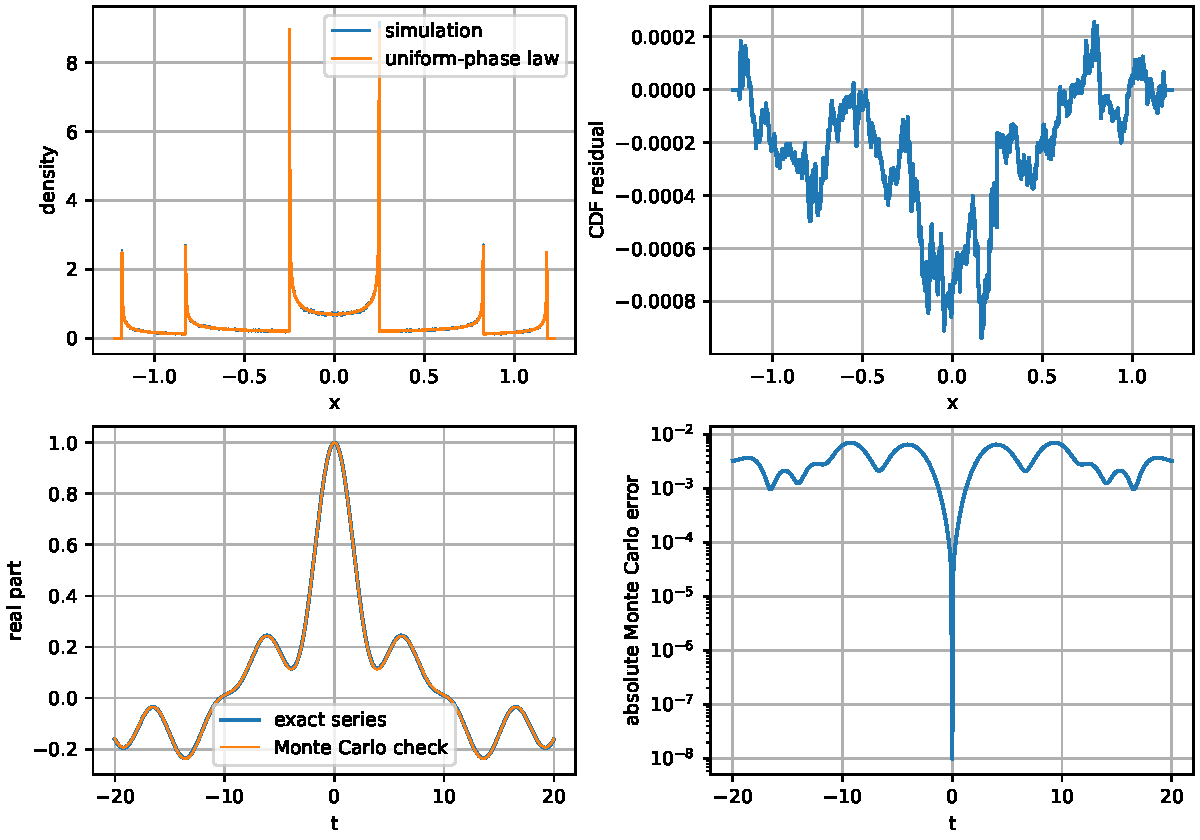
\includegraphics[width=.95\textwidth]{initial_distribution_comparison.pdf}
\caption{Density, CDF, and characteristic-function comparisons.}\label{fig:distribution}\end{figure}
\begin{figure}[htbp]\centering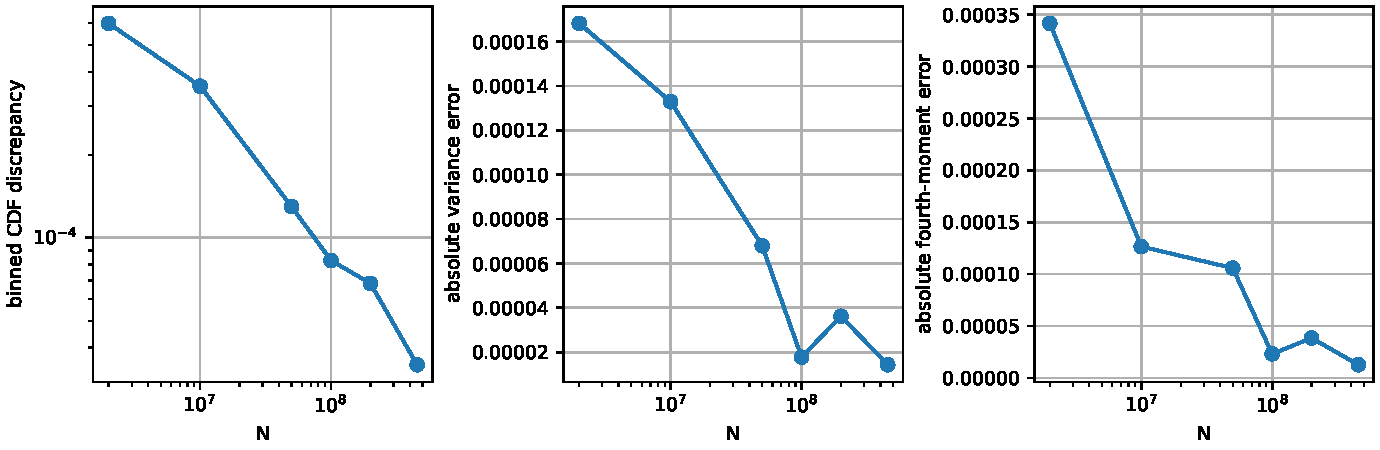
\includegraphics[width=.95\textwidth]{arithmetic_prefix_convergence.pdf}
\caption{Streaming prefix diagnostics through the full file.}\label{fig:prefix}\end{figure}
\section{Photonic realization: the Dutt et al. experiment}
\label{sec:dutt}
\subsection{Experimental input and scope}\label{subsec:dutt_input}
Dutt et al. realized a synthetic frequency lattice in an electro-optically modulated
fiber-ring resonator and measured its band structure directly in the time domain
\cite{DuttEtAl2019}.  Their platform supports reconfigurable long-range hopping and a
photonic gauge phase.  For the nonreciprocal experiment in their Fig.~4(c), the published
drive is
\begin{equation}
 V_M(t)=V_1\cos(\Omega_Rt)+V_2\cos(2\Omega_Rt+\phi),\qquad
 \frac{V_2}{V_1}=0.40,\qquad \phi=\frac{\pi}{2}.
\label{eq:dutt_drive}
\end{equation}
The experiment displayed a band strongly asymmetric about zero quasimomentum.  The same
work also showed, for nearest-neighbor hopping, that time-averaged transmission measures
the photonic density of states (DOS), including finite-linewidth-broadened Van Hove edges.

We make a \emph{published-parameter reconstruction}, not a fit to raw observations.
The supporting raw data are not deposited with the article; its data-availability
statement makes them available from the corresponding author on reasonable request.
In particular, Fig.~\ref{fig:dutt_reconstruction} contains no digitized experimental
points.  It states exactly which consequences follow from the reported harmonic drive and
which curves are predictions of the enlarged family.

\subsection{Exact map into the harmonic family}\label{subsec:dutt_map}
In the effective tight-binding description, write the two-range dispersion, in units of
the first-harmonic energy scale $A$, as
\begin{equation}
 \frac{\varepsilon_\phi(k)}{A}
 =\cos k+\alpha\cos(2k+\phi),\qquad
 \alpha=\frac{|J_2|}{|J_1|}.
\label{eq:dutt_dispersion_general}
\end{equation}
At $\phi=\pi/2$, reflection $k\mapsto-k$ turns
$\cos k-\alpha\sin(2k)$ into
\begin{equation}
 h_\alpha(k)=\cos k+\alpha\sin(2k).
\label{eq:dutt_harmonic}
\end{equation}
Consequently, the uniform-quasimomentum DOS in this model is exactly the $q=1$ member of
\eqref{eq:X} with
\begin{equation}
 (\lambda,\eta;r,s)=(\alpha,1;2,1),
\label{eq:dutt_parameter_map}
\end{equation}
up to the overall energy scale $A$.  Identifying the reported voltage ratio with
$\alpha=0.40$ uses the linear modulation-to-hopping calibration of the effective
two-harmonic model; if calibrated hopping amplitudes differ from the voltage ratio, the
same formulas apply after replacing $0.40$ by $|J_2/J_1|$.

\begin{table}[htbp]
\centering
\begin{tabular}{lll}\toprule
Experimental object & Harmonic-family object & Mathematical role\\ \midrule
$k=\Omega_Rt$ modulo $2\pi$ & $\Theta$ & uniform quasimomentum\\
nearest-neighbor hopping & $\eta\cos(s\Theta)$ & $s=1$, energy scale $A$\\
second-neighbor hopping & $\lambda\sin(r\Theta)$ & $r=2$, ratio $\lambda/\eta=\alpha$\\
gauge phases $\pm\pi/2$ & $M=\mp1$ & time-reversed homogeneous domains\\
inactive second harmonic & $M=0$ & cosine/arcsine domain\\
\bottomrule
\end{tabular}
\caption{Dictionary between the photonic effective model and the probabilistic
family.  The last three rows describe a possible ensemble protocol, not sitewise
disorder and not a claim about the single device in \cite{DuttEtAl2019}.}
\label{tab:dutt_dictionary}
\end{table}

\subsection{Calibration, broadening, and active-fraction recovery}
\label{subsec:dutt_sensitivity}
The following stability statement quantifies the scope of the published-parameter
reconstruction.  Let $d_{\mathbb T}$ denote circular distance modulo $2\pi$ and let
$W_1$ be the $1$-Wasserstein distance.
\begin{theorem}[Photonic calibration and broadening stability]
\label{thm:dutt_stability}
For $K\sim\operatorname{Unif}[0,2\pi)$, define
\begin{equation}
 E_{\alpha,\phi}=\cos K+\alpha\cos(2K+\phi),\qquad \alpha\ge0.
 \label{eq:dutt_stability_band}
\end{equation}
Then
\begin{equation}
 W_1\!\left(\mathcal L(E_{\alpha,\phi}),
             \mathcal L(E_{\alpha_0,\phi_0})\right)
 \le |\alpha-\alpha_0|+\alpha_0d_{\mathbb T}(\phi,\phi_0).
 \label{eq:dutt_wasserstein_calibration}
\end{equation}
The same right-hand side bounds the Hausdorff distance between the two band supports.
If an independent measurement error $Z$ is added, then
\begin{equation}
 W_1\!\left(\mathcal L(E_{\alpha,\phi}+Z),
             \mathcal L(E_{\alpha_0,\phi_0})\right)
 \le |\alpha-\alpha_0|+\alpha_0d_{\mathbb T}(\phi,\phi_0)
      +\mathbb E|Z|.
 \label{eq:dutt_wasserstein_noise}
\end{equation}
For $Z\sim N(0,\sigma^2)$, the last term equals
$\sigma\sqrt{2/\pi}$.
\end{theorem}
\begin{proof}
Couple both bands with the same $K$.  The elementary inequality
$|\cos u-\cos v|\le d_{\mathbb T}(u,v)$ gives
\begin{equation}
 |E_{\alpha,\phi}-E_{\alpha_0,\phi_0}|
 \le |\alpha-\alpha_0|+alpha_0d_{\mathbb T}(\phi,\phi_0).
 \label{eq:dutt_pointwise_calibration_bound}
\end{equation}
Taking expectations proves \eqref{eq:dutt_wasserstein_calibration}.  For any two
continuous functions on the same compact domain, a uniform bound on their difference
bounds the Hausdorff distance between their images, proving the support assertion.
Couple the noisy variable by adding $Z$ only to the first component and apply the
triangle inequality to obtain \eqref{eq:dutt_wasserstein_noise}.  The Gaussian absolute
first moment is $\sigma\sqrt{2/\pi}$.
\end{proof}

The active-domain fraction remains estimable after calibrated Gaussian broadening.
Let
\begin{equation}
 C_0(t)=J_0(t),\qquad
 C_{\alpha,\phi}(t)=\frac1{2\pi}\int_0^{2\pi}
 e^{it\{\cos k+\alpha\cos(2k+\phi)\}}\,dk,qquad
 \Delta(t)=C_{\alpha,\phi}(t)-C_0(t).
 \label{eq:dutt_active_inactive_cf}
\end{equation}
\begin{theorem}[Exact one-frequency estimator under Gaussian broadening]
\label{thm:dutt_q_estimator}
Let $X_1,\ldots,X_N$ be i.i.d. from the homogeneous-domain mixture that selects
$\cos K$ with probability $1-q$ and $E_{\alpha,\phi}$ with probability $q$.  Observe
$Y_j=X_j+Z_j$, where the $Z_j$ are independent $N(0,\sigma^2)$ variables and
$\alpha,\phi,\sigma$ are known.  For a fixed $t\ne0$ with $\Delta(t)\ne0$, put
\begin{equation}
 \widehat q_N(t)=
 \frac{\operatorname{Re}\!\left[
 \{e^{\sigma^2t^2/2}\widehat\phi_{Y,N}(t)-C_0(t)\}
 \overline{\Delta(t)}\right]}{|\Delta(t)|^2}.
 \label{eq:dutt_q_estimator}
\end{equation}
Then $\mathbb E\widehat q_N(t)=q$, $\widehat q_N(t)\to q$ almost surely, and
\begin{equation}
 \sqrt N\{\widehat q_N(t)-q\}
 \Longrightarrow N\!\left(0,
 \operatorname{Var}\!\left[
 \frac{\operatorname{Re}\{e^{\sigma^2t^2/2}e^{itY_1}
 \overline{\Delta(t)}\}}{|\Delta(t)|^2}\right]\right).
 \label{eq:dutt_q_estimator_clt}
\end{equation}
\end{theorem}
\begin{proof}
Independence and the Gaussian characteristic function give
\begin{equation}
 e^{\sigma^2t^2/2}\mathbb E e^{itY_1}
 =C_0(t)+q\Delta(t).
 \label{eq:dutt_deconvolved_cf_identity}
\end{equation}
Substitution into \eqref{eq:dutt_q_estimator} proves unbiasedness.  The strong law
applied to the bounded complex variables $e^{itY_j}$ proves almost-sure consistency.
Finally, \eqref{eq:dutt_q_estimator} is an affine function of the sample mean of bounded
real variables.  The ordinary central limit theorem gives
\eqref{eq:dutt_q_estimator_clt}.
\end{proof}

A seeded audit with $q=0.65$, $N=2000$, and 300 replications confirms the distinction
between known Gaussian broadening and hopping miscalibration.  At measurement width
$\sigma/A=0.05$, the mean estimates of $q$ were $0.916$, $0.651$, and $0.509$ when the
nominal hopping ratios were respectively $0.32$, $0.40$, and $0.48$, while the true
ratio was $0.40$.  Thus the analytic deconvolution removes known Gaussian attenuation,
but a $20\%$ hopping error produces substantial model bias.  This is precisely why a
future comparison with raw spectra must calibrate $|J_2/J_1|$ rather than identify it
automatically with a voltage ratio.
\begin{figure}[htbp]
\centering
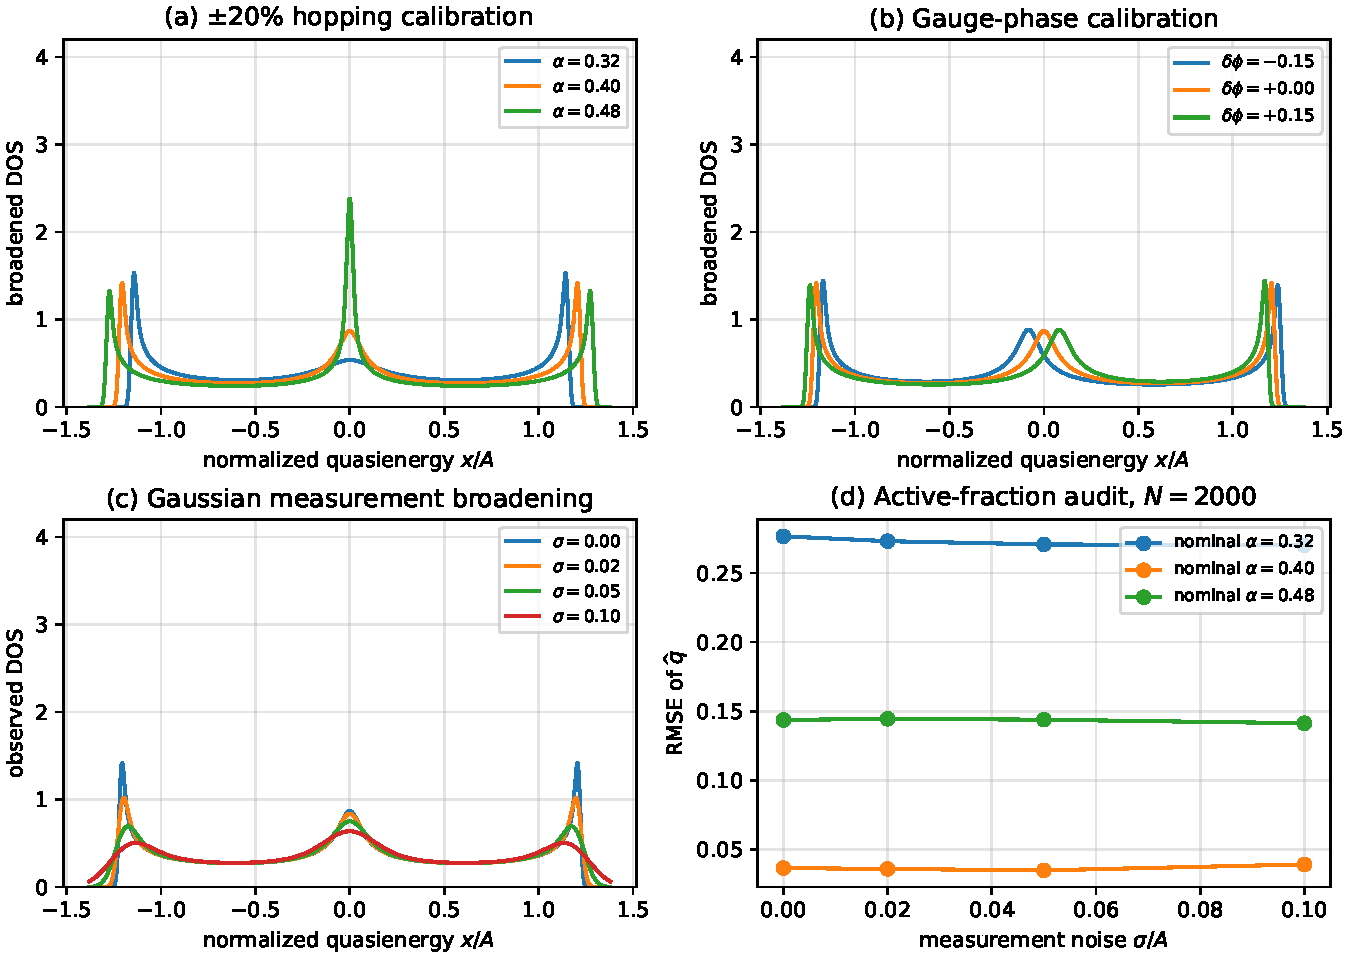
\includegraphics[width=\textwidth]{dutt2019_sensitivity_audit.pdf}
\caption{Sensitivity of the Dutt published-parameter reconstruction.  (a) DOS under a
$\pm20\%$ hopping-ratio change.  (b) Gauge-phase offsets.  (c) Gaussian measurement
broadening.  (d) RMSE of the exact one-frequency active-fraction estimator under correct
and misspecified hopping calibration.  All curves are model calculations, not fits to
experimental raw data.}
\label{fig:dutt_sensitivity}
\end{figure}

\subsection{A nearby, testable singularity transition}\label{subsec:dutt_threshold}
The published ratio lies close to a sharp change in critical-point topology.
\begin{proposition}\label{prop:dutt_threshold}
For $h_\alpha$ in \eqref{eq:dutt_harmonic}, let $\alpha>0$.  If
$0<\alpha<1/2$, there are two nondegenerate critical points per period.  At
$\alpha=1/2$, a cubic stationary point occurs at $k=3\pi/2$ and produces a DOS
singularity proportional to $|x|^{-2/3}$.  If $\alpha>1/2$, this point splits into
two additional nondegenerate critical points, producing an additional pair of critical
values.
\end{proposition}
\begin{proof}
With $u=\sin k$, the stationary equation is
\begin{equation}
 4\alpha u^2+u-2\alpha=0,\qquad
 u_\pm=\frac{-1\pm\sqrt{1+32\alpha^2}}{8\alpha}.
\label{eq:dutt_stationary_roots}
\end{equation}
The root $u_+$ is always admissible, whereas $u_-$ enters $[-1,1]$ precisely at
$\alpha=1/2$, when $u_-=-1$.  Direct differentiation gives
$h'_{1/2}(3\pi/2)=h''_{1/2}(3\pi/2)=0$ and
$h'''_{1/2}(3\pi/2)\ne0$.  Theorem~\ref{thm:singularity} supplies the exponent.
\end{proof}
\begin{proposition}[Quantitative unfolding of the cubic transition]
\label{prop:dutt_cubic_unfolding}
Put $\alpha=1/2+\delta$ with $\delta>0$.  The cubic phase $3\pi/2$ splits into
two ordinary critical phases
\begin{equation}
 k_\pm=\frac{3\pi}{2}\pm\frac{2}{\sqrt3}\delta^{1/2}
       +O(\delta^{3/2}).
 \label{eq:dutt_split_phases}
\end{equation}
Their critical values and curvatures satisfy
\begin{align}
 h_\alpha(k_\pm)
 &=\mp\frac{8}{3\sqrt3}\delta^{3/2}+O(\delta^{5/2}),
 \label{eq:dutt_split_energies}\\
 |h_\alpha''(k_\pm)|
 &=2\sqrt3\,\delta^{1/2}+O(\delta^{3/2}).
 \label{eq:dutt_split_curvatures}
\end{align}
Consequently, the separation of the two new singular energies is
\begin{equation}
 \frac{16}{3\sqrt3}\delta^{3/2}+O(\delta^{5/2}),
 \label{eq:dutt_energy_resolution_scale}
\end{equation}
and the local quadratic-DOS prefactor at either new phase is
\begin{equation}
 \frac{q}{2\pi\,3^{1/4}}\delta^{-1/4}\{1+O(\delta)\}.
 \label{eq:dutt_prefactor_unfolding}
\end{equation}
\end{proposition}
\begin{proof}
Write $k=3\pi/2+u$.  Uniformly for small $u$ and $\delta$,
\begin{equation}
 h_{1/2+\delta}(3\pi/2+u)
 =-2\delta u+\left(\frac12+\frac43\delta\right)u^3
  +O(u^5+\delta u^5).
 \label{eq:dutt_cubic_normal_form}
\end{equation}
Differentiation and solution of the two nonzero stationary branches give
$u_\pm=\pm2\delta^{1/2}/\sqrt3+O(\delta^{3/2})$, proving
\eqref{eq:dutt_split_phases}.  Substitution into
\eqref{eq:dutt_cubic_normal_form} proves \eqref{eq:dutt_split_energies}; differentiating
twice proves \eqref{eq:dutt_split_curvatures}.  Subtraction gives
\eqref{eq:dutt_energy_resolution_scale}.  Finally, Theorem~\ref{thm:singularity} with
$m=2$, $a_2=h_\alpha''(k_\pm)/2$, and $N_2=2$ gives the prefactor
$q(2/|h_\alpha''(k_\pm)|)^{1/2}/(2\pi)$, which is
\eqref{eq:dutt_prefactor_unfolding}.
\end{proof}
Equation~\eqref{eq:dutt_energy_resolution_scale} supplies an explicit resolution scale.
If the dimensionless linewidth is $\Gamma/A$, resolving the two new peaks requires it
to be small relative to
$16\delta^{3/2}/(3\sqrt3)$; the statement is a scale requirement derived from the band,
not a claim about the linewidth achieved in \cite{DuttEtAl2019}.
At the reported value $\alpha=0.40$, the active-domain band therefore has only its two
ordinary edge critical values,
\begin{equation}
 x_\mathrm{edge}/A=\pm1.2146735483.
\label{eq:dutt_edges}
\end{equation}
The critical ratio $0.50$ is a prospective experimental target: tuning through it should
create a central higher-order DOS anomaly and then split it.  This statement is a model
prediction, not a reported observation in \cite{DuttEtAl2019}.

\begin{figure}[htbp]
\centering
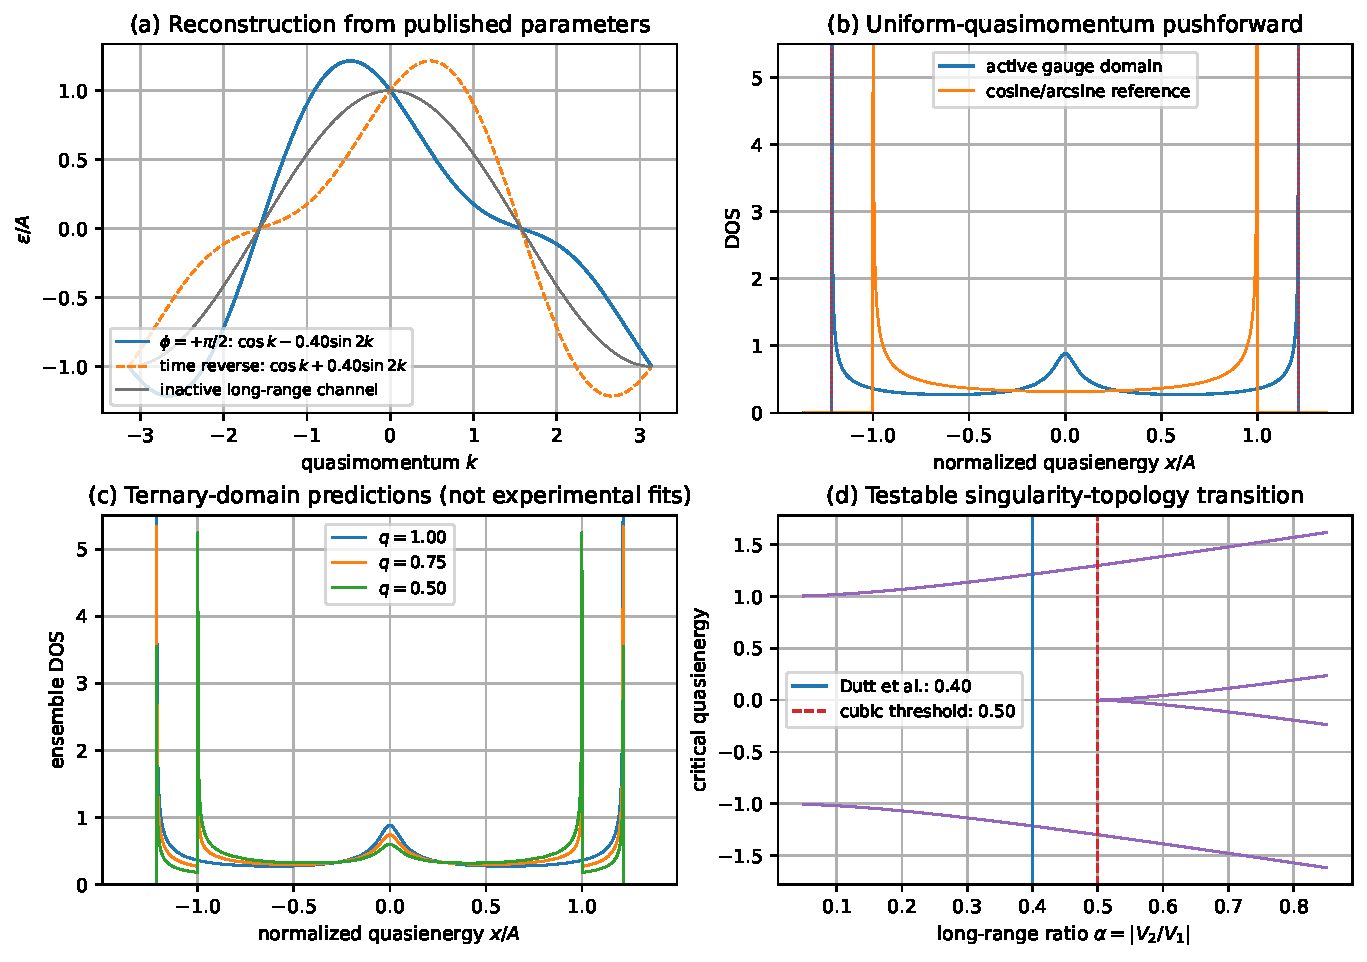
\includegraphics[width=\textwidth]{dutt2019_family_reconstruction.pdf}
\caption{Application to the published parameters of Dutt et al.
(a) The $\phi=\pi/2$ band and its time reverse; their pushforward laws coincide.
(b) Phase-grid evaluation of the corresponding DOS and the inactive cosine reference.
(c) Predictions for homogeneous-domain ensembles; these are not experimental fits.
(d) Critical values versus second-neighbor ratio, showing the experimental value $0.40$
and the predicted cubic threshold $0.50$.}
\label{fig:dutt_reconstruction}
\end{figure}

\subsection{What the generalization adds}\label{subsec:dutt_extension}
The fixed-gauge experiment corresponds to a single homogeneous branch.  The ternary gate
becomes physical for an ensemble of independently prepared homogeneous domains:
\begin{equation}
 \frac{\varepsilon_M(k)}A=\cos k+\alpha M\sin(2k),\qquad
 P(M=0)=1-q,\quad P(M=\pm1)=q/2.
\label{eq:dutt_domain_ensemble}
\end{equation}
Here $M=\pm1$ represents balanced opposite gauge phases and $M=0$ an inactive
long-range drive.  The ensemble DOS is then exactly
\begin{equation}
 f_q(x)=(1-q)f_{\mathrm{cos}}(x)+qf_{\mathrm{active}}(x),
\label{eq:dutt_ensemble_dos}
\end{equation}
so $q$ is the active-domain fraction.  This extension gives simultaneously an analytic DOS, its critical exponents, and a
topology diagram in $\alpha$, with $q$ interpreted as the active-domain fraction.  These
are model consequences of \eqref{eq:dutt_domain_ensemble}; they are not observations
reported in \cite{DuttEtAl2019}.  The construction does not assert that the device has
random sitewise hopping.  An operational homogeneous-domain protocol would repeat a full
band acquisition with one global drive setting held fixed during each acquisition:
$+\pi/2$, $-\pi/2$, or second-harmonic off.  Pooling complete acquisitions in proportions
$q/2,q/2,1-q$ produces \eqref{eq:dutt_ensemble_dos}.  It differs from sitewise disorder,
which would randomize hopping from site to site within a single acquisition and would
not be described by the mixture identity \eqref{eq:dutt_ensemble_dos}.

\section{Homogeneous-domain interpretation}\label{sec:physics}
For a homogeneous domain indexed by $M$, take range-$s$ hopping $t_s=\eta/2$ and
range-$r$ hopping $t_r=-i\lambda M/2$.  The Hermitian Bloch dispersion is
\begin{equation}\varepsilon_M(k)=t_se^{isk}+\overline t_se^{-isk}+t_re^{irk}+\overline t_re^{-irk}
=\eta\cos(sk)+\lambda M\sin(rk).\label{eq:dispersion}\end{equation}
Thus \eqref{eq:X} is an ensemble of homogeneous domains with uniform quasimomentum.
It is not sitewise disorder.  The $M=\pm1$ domains are conjugate and have the same DOS.
The imaginary hopping is a Hermitian Peierls phase, not by itself non-Hermitian
nonreciprocity.  Photonic or Floquet relevance requires a platform-specific derivation.
\begin{thebibliography}{99}
\bibitem{BergelsonKulagaPrzymusLemanczykRichter2019}
V. Bergelson, J. Kułaga-Przymus, M. Lemańczyk, and F. K. Richter,
A generalization of Kátai's orthogonality criterion with applications,
\emph{Discrete Contin. Dyn. Syst.} 39 (2019), no.~5, 2581--2612,
doi:10.3934/dcds.2019108.
\bibitem{ClassenBetouras2025} L. Classen and J. J. Betouras, High-order Van Hove singularities and their connection to flat bands, \emph{Annu. Rev. Condens. Matter Phys.} 16 (2025), 229--251, doi:10.1146/annurev-conmatphys-042924-015000, arXiv:2405.20226.
\bibitem{CarrascoFlorens2000}
M. Carrasco and J.-P. Florens,
Generalization of GMM to a continuum of moment conditions,
\emph{Econometric Theory} 16 (2000), no.~6, 797--834,
doi:10.1017/S0266466600166010.
\bibitem{FeuervergerMcDunnough1981}
A. Feuerverger and P. McDunnough,
On the efficiency of empirical characteristic function procedures,
\emph{J. Roy. Statist. Soc. Ser. B} 43 (1981), no.~1, 20--27.
\bibitem{GrahamKolesnik1991}
S. W. Graham and G. Kolesnik,
\emph{Van der Corput's Method of Exponential Sums},
London Mathematical Society Lecture Note Series 126,
Cambridge University Press, Cambridge, 1991,
doi:10.1017/CBO9780511661976.
\bibitem{KuipersNiederreiter1974}
L. Kuipers and H. Niederreiter,
\emph{Uniform Distribution of Sequences},
Wiley-Interscience, New York, 1974.
\bibitem{MatomakiShaoTaoTeravainen2023}
K. Matom\"aki, X. Shao, T. Tao, and J. Ter\"av\"ainen,
Higher uniformity of arithmetic functions in short intervals I. All intervals,
\emph{Forum Math. Pi} 11 (2023), e29,
doi:10.1017/fmp.2023.28, arXiv:2204.03754v4.
\bibitem{DLMF2026} NIST Digital Library of Mathematical Functions, Chapter 10, \url{https://dlmf.nist.gov/10}, accessed 2026-07-13.
\bibitem{DuttEtAl2019} A. Dutt, M. Minkov, Q. Lin, L. Yuan, D. A. B. Miller, and S. Fan,
Experimental band structure spectroscopy along a synthetic dimension,
\emph{Nature Communications} 10 (2019), Article 3122,
doi:10.1038/s41467-019-11117-9.
\bibitem{Massart1990}
P. Massart,
The tight constant in the Dvoretzky--Kiefer--Wolfowitz inequality,
\emph{Ann. Probab.} 18 (1990), no.~3, 1269--1283,
doi:10.1214/aop/1176990746.
\bibitem{Serfling1974}
R. J. Serfling,
Probability inequalities for the sum in sampling without replacement,
\emph{Ann. Statist.} 2 (1974), no.~1, 39--48,
doi:10.1214/aos/1176342611.
\bibitem{VanHove1953} L. Van Hove, The occurrence of singularities in the elastic frequency distribution of a crystal, \emph{Phys. Rev.} 89 (1953), 1189--1193, doi:10.1103/PhysRev.89.1189.
\end{thebibliography}
\end{document}
